%*******************************************************************************
%*********************************** Second Chapter ****************************
%*******************************************************************************

\chapter{Background}
\label{chap2}

In this chapter, we provide an overview of the preliminaries for comprehending the methodology in the included papers in this thesis. We assume that the reader has some basic knowledge in calculus, linear algebra, and probability theory. Section \ref{sec:problem_settings_in_ml} gives an introduction to machine learning, including different problem settings, some terminology, as well as the notation that will be used throughout this thesis. In Section \ref{sec:deep_learning}, we give an overview of deep learning~\cite{goodfellow2016deep}, where we cover the different types of network architectures that has been used in the thesis, as well as a brief introduction to deep reinforcement learning. 

%The goal with this chapter is to provide the reader with preliminaries that are useful for comprehending the included papers. We assume that the reader has some knowledge in calculus, linear algebra, and probability theory, but we intend to keep it on a basic level. First, we give the notation that will be used throughout the thesis. Then, we will introduce a selection of related works to place the thesis into context. 

%\MK{What is chapter about? Add references to sections! We focus on deep learning architectures rather than how they are trained.}



\section{Problem Settings in Machine Learning}\label{sec:problem_settings_in_ml}

Machine learning tasks can be divided into three main fields, namely, \textit{supervised learning}, \textit{unsupervised learning}, and \textit{reinforcement learning} (RL). In this section, we will give a brief introduction to these topics to provide some context on the challenges that we are addressing in this thesis. 

We will begin by introducing some algebraic notation that will be used throughout this thesis. For representing data, we use the vector $\vx$ which is a column vector 
\begin{align*}
	\vx = [x_1, \dots, x_D]^T,
\end{align*}
where $x_i$ for $1 \leq i \leq D$ is the $i$-th scalar, real-valued feature of the data vector, and the superscript $T$ transposes the row vector into a column vector. In some cases, each data vector $\vx$ have an assigned class label $y$ which is an integer number. Scalars can hence both represent real values and integers. The data vector $\vx$ will often represent a 2-dimensional image, where each feature $x_i$ is a pixel. In this thesis, we still however denote images as column vectors in our equations for simplicity. 

We assume that the data follows some underlying distribution, $p_{data}(\vx)$, usually referred to as the data generating distribution. In machine learning, we are often interested in approximating $p_{data}$ with a distribution $p_{\vtheta}(\vx)$ parameterized by $\vtheta$ given a finite dataset $\gD = \{\vx^{(i)}\}_{i=1}^{N}$ of $N$ samples where $\vx^{(i)} \sim p_{data}(\vx)$. Estimating the parameters $\vtheta$ from the dataset $\gD$ is called the \textit{training phase}. A central goal for most applications in machine learning is to make predictions on new data which is called \textit{generalization}. We measure the generalization capability by evaluating the task of interest on a held-out dataset during the \textit{test phase}.

\vspace{-3mm}
\paragraph{Supervised Learning.} In this setting, we are given a dataset $\{(\vx^{(i)}, y^{(i)})\}_{i=1}^{N}$ where each data point $\vx^{(i)}$ is accompanied with a target $y^{(i)}$. In classification problems, the target $y \in \{1, \dots, C\}$ belongs to one of $C$ discrete categories, while in regression problems, the targets $y \in \R$ are continuous and real-valued. The goal is to estimate $p_{\vtheta}(y | \vx)$ which is the probability of assigning the target $y$ given data $\vx$. We represent $p_{\vtheta}(y | \vx) = f_{\vtheta}(x)$ with the parameterized function $f_{\vtheta}(x)$ which maps data $\vx$ to target variables $y$.  

%a function $f_{\vtheta}(\vx)$ that assigns the correct target to each example in the training set as accurately as possible. In classification problems, each target belongs to one of $K$ discrete categories, such that $\vy = \{1, \dots, K\}$, and we want to predict which of the categories that new data belongs to. Classification tasks will be involved in all included papers of this thesis wherein Paper \ref{chap:paperA} and B we focus on assigning the correct product category to images of grocery items. Another problem type in supervised learning is regression where the targets are continuous and real-valued. An example of a regression task is to predict the outdoors temperature tomorrow given the observed temperature today. 

\vspace{-3mm}
\paragraph{Unsupervised Learning.} The goal in the unsupervised setting is to reveal hidden structures in the given dataset $\{\vx^{(i)}\}_{i=1}^{N}$ without access to target variables. For example, we might be interested in estimating the data generating distribution $p_{data}$ with $p_{\vtheta}$ (as mentioned above), discovering groups of similar data points using clustering techniques, or project high-dimensional data into two or three dimensions for visualization purposes. 

%Here, we are given a dataset $\{\vx^{(i)}\}_{i=1}^{N}$ without access to any corresponding targets. The goal in this unsupervised setting may then be to find hidden structures in the given dataset. For example, we might be interested in discovering groups of similar examples with \textit{clustering} techniques, or we may want to use \textit{density estimation} where we approximate the true data distribution $p_{data}$ with a parametric distribution $p_{\vtheta}$ using the collected dataset, or we may want to project high-dimensional data into two or three dimensions for \textit{visualization} purposes. We will get back to these goals when we introduce representation learning in Section X. 

\vspace{-3mm}
\paragraph{Reinforcement Learning.} For these problems, we have a \textit{learning agent}
that performs actions based on perceived states of the environment to reach some specific goal represented by a reward signal $r$. An example of such a task is the Mountain Car problem~\cite{sutton2018reinforcement} where the agent tries to drive a car over the top of a hill. The action selection is modeled by the policy $\pi_{\vtheta}(a | \vs)$ which is a mapping from states $\vs$ to actions $a$. The goal for the agent is to learn a policy that maximizes the reward within a specified time limit. 


%For these problems, we have a \textit{learning agent} that wants reach a goal in an environment by performing a given set of actions. After performing an action, the agent observes the state of the environment and receives a reward from the environment saying how good or bad the taken action was to reach the goal. The objective for the agent is to maximize the reward signal within the time the agent reaches the goal. The agent then has to learn a policy for deciding which actions to perform in certain situations in the environment. The policy $\pi_{\vtheta}(\va | \vs)$ is a mapping from perceived states $\vs$ in the environment to actions $\va$ that should maximize the reward signal. An example of a task that can be framed as a RL problem is the so called Mountain Car problem, where the agent is a car that is trying to drive up to the top of a hill. The state represents the position and velocity of the car and the agent must take actions that will move the car forward or backwards. The objective is to reach the goal with as little time as possible, and the agent is encouraged to do so by the environment by sending the agent a negative reward for every time step that passes without reaching the top of the hill. We will return to the RL framework later when we describe the prerequisites for Paper D. \vspace{1mm}

\begin{comment}
\section{Notation and Terminology}\label{sec:notation}

We will begin by introducing some algebraic notation that will be used throughout this thesis. For representing data, we use the vector $\vx$ which is a column vector 
\begin{align*}
	\vx = [x_1, \dots, x_D]^T,
\end{align*}
where $x_i$ for $1 \leq i \leq D$ is the $i$-th scalar, real-valued feature of the data vector, and the superscript $T$ transposes the column vector into a row vector. In some cases, each data vector $\vx$ have an assigned class label $y$ which is an integer number. Scalars can hence both represent real values and integers. The data vectors $\vx$ will often represent a 2-dimensional image, where each feature $x_i$ is a pixel, in this thesis, but we still represent images as column vectors for simplicity. 


%We will begin by providing some algebraic notation that will be used for representing various types of data in the thesis. Scalars (both integer and real) are denoted by italic letters such as $a$. Vectors are denoted by lowercase bold italic letters such as $\vx$, where all vectors are assumed to be column vectors. A superscript $T$ denotes the transpose of a vector or matrix, such that $\vx^{T}$ becomes a row vector. Matrices are denoted as uppercase bold italic letters such as $\mW$. The notation $(w_1, \dots, w_m)$ denotes a row vector with $m$ elements, where the corresponding column vector is denoted as $(w_1, \dots, w_m)^{T}$. 

We assume that the data follows some underlying distribution, $p_{data}(\vx)$, usually referred to as the data generating distribution. In machine learning, we are often interested in approximating $p_{data}$ with a distribution $p_{\vtheta}(\vx)$ parameterized by $\vtheta$ given a finite dataset $\gD = \{\vx^{(i)}\}_{i=1}^{N}$ of $N$ samples where $x^{(i)} \sim p_{data}(\vx)$. Estimating the parameters $\vtheta$ from the dataset $\gD$ is called the \textit{training phase}. A central goal for most applications in machine learning is to make predictions on new data which is called \textit{generalization}. We measure the generalization capability by evaluating the task of interest on a held-out dataset during the \textit{test phase}.


%A dataset is denoted by the set $\gD = \{\vx^{(1)}, \dots, \vx^{(N)} \}$, where $\vx^{(i)}$ is the $i$-th example among the $N$ data points. Each data point is assumed to belong in a space of vectors denoted by $\gX$, such that $\vx \in \gX$. The data generating distribution is denoted by $p_{data}(\gX)$ which is usually unknown. To provide an example, we let the vector $\vx = (x_1, \dots, x_m)$ represent a flattened image of $m$ pixels. In this case, all possible images that can exist belong to the space $\gX$ and the data generating distribution $p_{data}(\gX)$ gives the probability of how likely each image is to occur in the world. In supervised learning, there is also a target, either denoted as $y^{(i)}$ or $\vy^{(i)}$, associated with $\vx^{(i)}$. The target belongs to the target space $\gY$, where the space is discrete $\gY = \{1, \dots, C\}$ for classification tasks over $C$ number of classes, or continuous $\gY = (-\infty, \infty)$ over an interval of real values for regression tasks. 


%Throughout this thesis, we take a machine learning approach to solve tasks by tuning an adaptive model using a dataset called the \textit{training set}. In our case, we will represent the model with a function $f_{\vtheta}(\vx)$ that allows us to predict outcomes of events/data $\vx$ from the task of interest. The parameters $\vtheta$ expresses the function and we use machine learning algorithms for tuning parameters with the given dataset during the training phase. Once the model is trained, we often enter the \textit{test phase} where we want to evaluate the model by predicting outcomes on an unseen dataset called the \textit{test set}. The ability to predict outcomes of new data that is different from the examples seen during training is called \textit{generalization}, which is a central goal for most applications in machine learning and pattern recognition. 


\section{Problem Settings in Machine Learning}

Machine learning problems can be divided into three main fields, namely, \textit{supervised learning}, \textit{unsupervised learning}, and \textit{reinforcement learning} (RL). Since this thesis includes work from each of these problem settings, we will briefly introduce these topics to provide the reader with context on the tasks that we are trying to solve. 

\MK{TO-DO: Add references to papers and sections!}
\paragraph{Supervised Learning.} In this setting, we are given a dataset $\{(\vx^{(i)}, \vy^{(i)})\}_{i=1}^{N}$ where each data example $\vx^{(i)}$ is accompanied with a target $\vy^{(i)}$. The goal is to estimate a function $f_{\vtheta}(\vx)$ that assigns the correct target to each example in the training set as accurately as possible. In classification problems, each target belongs to one of $K$ discrete categories, such that $\vy = \{1, \dots, K\}$, and we want to predict which of the categories that new data belongs to. Classification tasks will be involved in all included papers of this thesis wherein Paper \ref{chap:paperA} and B we focus on assigning the correct product category to images of grocery items. Another problem type in supervised learning is regression where the targets are continuous and real-valued. An example of a regression task is to predict the outdoors temperature tomorrow given the observed temperature today. 

\paragraph{Unsupervised Learning.} Here, we are given a dataset $\{\vx^{(i)}\}_{i=1}^{N}$ without access to any corresponding targets. The goal in this unsupervised setting may then be to find hidden structures in the given dataset. For example, we might be interested in discovering groups of similar examples with \textit{clustering} techniques, or we may want to use \textit{density estimation} where we approximate the true data distribution $p_{data}$ with a parametric distribution $p_{\vtheta}$ using the collected dataset, or we may want to project high-dimensional data into two or three dimensions for \textit{visualization} purposes. We will get back to these goals when we introduce representation learning in Section X. 

\paragraph{Reinforcement Learning.} For these problems, we have a \textit{learning agent} that wants reach a goal in an environment by performing a given set of actions. After performing an action, the agent observes the state of the environment and receives a reward from the environment saying how good or bad the taken action was to reach the goal. The objective for the agent is to maximize the reward signal within the time the agent reaches the goal. The agent then has to learn a policy for deciding which actions to perform in certain situations in the environment. The policy $\pi_{\vtheta}(\va | \vs)$ is a mapping from perceived states $\vs$ in the environment to actions $\va$ that should maximize the reward signal. An example of a task that can be framed as a RL problem is the so called Mountain Car problem, where the agent is a car that is trying to drive up to the top of a hill. The state represents the position and velocity of the car and the agent must take actions that will move the car forward or backwards. The objective is to reach the goal with as little time as possible, and the agent is encouraged to do so by the environment by sending the agent a negative reward for every time step that passes without reaching the top of the hill. We will return to the RL framework later when we describe the prerequisites for Paper D. \vspace{1mm}

There exist many different methods for solving problems within these three fields. In this thesis, we employ deep learning methods which has been successfully applied in each field by representing the models with deep neural networks~\cite{he2016deep, bengio2013representation, mnih2015human}.

%that is trying to maximize a reward signal $r$ by performing a given set of actions in an environment to reach a specific goal. The agent observes the state of the environment 


%In this paradigm, we are concerned with decision-making where the goal is to take actions that maximize some reward. The decision-making is modeled by a policy which bases the action selection on observations that are collected by interacting with the task environment through the selected actions. One main challenge is how to handle the trade-off between exploration of different actions in new situations and exploitation by selecting actions where the agent already has experienced good reward signals. Furthermore, the reward signal can be received either in dense or sparse forms, where sparse rewards are typically more challenging to learn from and are less sample-efficient. 
\end{comment}

\section{Deep Learning}\label{sec:deep_learning}

In this section, we give an introduction to deep learning~\cite{goodfellow2016deep} which is a family of machine learning methods used in this thesis. Deep learning methods are capable of learning tasks from large and high-dimensional datasets thanks to larger volumes of available training data, more efficient machine learning algorithms, and advances in computer hardware in the last decades. A deep learning architecture is constructed by stacking layers of non-linear mapping functions that give intermediate representations of the input data, where the last layer usually outputs a predicted target answer from the queried input. This approach has been successfully applied in various number of fields such as computer vision~\cite{he2016deep, krizhevsky2012imagenet}, natural language processing~\cite{devlin2018bert}, and reinforcement learning~\cite{mnih2015human, silver2016mastering}. 

%In this section, we give an introduction to deep learning~\cite{goodfellow2016deep} which is a family of machine learning methods that we have used in this thesis. Deep learning methods are capable of learning tasks from large and high-dimensional datasets due to more efficient machine learning algorithms and advances in computer hardware in the last decades. A deep learning architecture is constructed by stacking layers of parameters that extract intermediate representations of the input data, where the last layer usually outputs a predicted target answer from the queried input. This approach has been successfully applied in various number of fields such as computer vision~\cite{he2016deep, krizhevsky2012imagenet}, natural language processing~\cite{devlin2018bert}, and reinforcement learning~\cite{mnih2015human, silver2016mastering}. 

Deep networks are most commonly optimized using the Stochastic Gradient Descent (SGD) algorithm. This procedure uses gradients of a loss function $\gL(f_{\vtheta}(\vx), \vy)$ with respect to every parameter to perform the update step
\begin{align}\label{eq:weight_update_sgd}
	\vtheta = \vtheta - \eta \nabla_{\vtheta} \gL(f_{\vtheta}(\vx), \vy),
\end{align} 
where $\eta$ is the learning rate which determines how much the weights should be updated with the computed gradient. Common loss functions $\gL$ are the cross-entropy loss for classification and the mean-squared error for regression tasks. The gradients are computed using the backpropagation algorithm~\cite{rumelhart1986learning} which estimates the gradients iteratively one layer at a time, going back and forth. To improve the computational efficiency, the mapping function parameters are estimated from the average of the gradients from a randomly sampled mini-batch of data. %which computes the gradients iteratively backwards one layer at a time. To improve the computational efficiency, we compute the average of the gradients from a randomly sampled mini-batch of data from the dataset during the parameter updates.

Many innovations have been designed in recent years to stabilize the training of deep neural network architectures. For instance, dropout~\cite{srivastava2014dropout} is used for mitigating overfitting to the training data by randomly making some layer outputs passive to encourage the parameters to take more (or less) responsibility for the inputs. %dropout~\cite{srivastava2014dropout} is used for mitigating overfitting to the training data by randomly keeping layer outputs active to encourage the parameters to take more (or less) responsibility for the inputs. 
Batch normalization~\cite{ioffe2015batch, santurkar2018does} normalizes the layer inputs to enable faster and more stable learning. Residual connections~\cite{he2016deep} eases training networks with hundreds of layers by mitigating the degradation problem, where adding more layers resulted in higher training error. Furthermore, various adaptive learning rate optimizers~\cite{kingma2014adam,liu2019variance,tieleman2012lecture} for the SGD updates, learning rate schedulers~\cite{smith2017cyclical}, and network initializations~\cite{glorot2010understanding, he2015delving} have been proposed to enable more efficient training. We refer the reader to the provided references for the details on these techniques.
Next, we will describe three popular types of neural networks that have been applied in the experiments of this thesis, namely, multilayer perceptrons (MLPs), convolutional neural networks (CNNs), and recurrent neural networks (RNNs).

\vspace{-3mm}
\begin{wrapfigure}{r}{0.39\textwidth}
	\centering
	\vspace{-3mm}
	\resizebox{0.39\textwidth}{!}{
		
    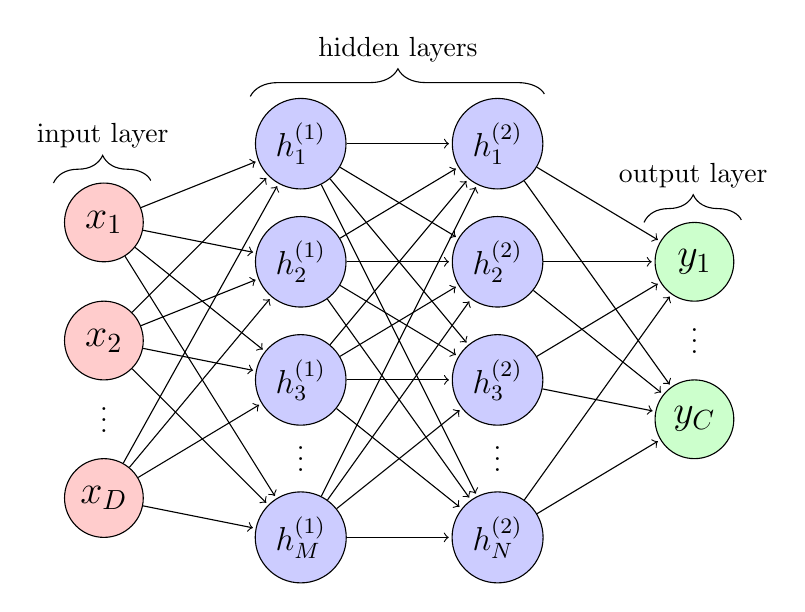
\begin{tikzpicture}[shorten >=1pt]
	\tikzstyle{unit}=[draw,shape=circle,minimum size=1.0cm]
	
	%\node[unit,fill=red!20](x1) at (0,5.0){\Large $x_1$};
	\node[unit,fill=red!20](x1) at (0,3.5){\Large $x_1$};
	\node[unit,fill=red!20](x2) at (0,2){\Large $x_2$};
	\node(dots) at (0,1.1){\vdots};
	\node[unit,fill=red!20](xd) at (0,0){\Large $x_D$};
	
	%\node[unit,fill=blue!20](w11) at (2.5,6.0){\large $h_1^{(1)}$};
	\node[unit,fill=blue!20](h11) at (2.5,4.5){\large $h_1^{(1)}$};
	\node[unit,fill=blue!20](h12) at (2.5,3.0){\large $h_2^{(1)}$};
	\node[unit,fill=blue!20](h13) at (2.5,1.5){\large $h_3^{(1)}$};
	\node(dots) at (2.5,0.6){\vdots};
	\node[unit,fill=blue!20](h1m) at (2.5,-0.5){\large $h_M^{(1)}$};
	
	%\node[unit,fill=blue!20](w21) at (5,6.0){\large $h_1^{(2)}$};
	\node[unit,fill=blue!20](h21) at (5,4.5){\large $h_1^{(2)}$};
	\node[unit,fill=blue!20](h22) at (5,3.0){\large $h_2^{(2)}$};
	\node[unit,fill=blue!20](h23) at (5,1.5){\large $h_3^{(2)}$};
	\node(dots) at (5,0.6){\vdots};
	\node[unit,fill=blue!20](h2n) at (5,-0.5){\large $h_N^{(2)}$};
	
	%\node[unit,fill=green!20](y1) at (7.5,4.5){\Large $y_1$};
	\node[unit,fill=green!20](y1) at (7.5,3.0){\Large $y_1$};
	\node(dots) at (7.5,2.1){\vdots};
	\node[unit,fill=green!20](yc) at (7.5,1.0){\Large $y_C$};
	
	% input to hidden1
	\draw[->] (x1) -- (h11);
	\draw[->] (x1) -- (h12);
	\draw[->] (x1) -- (h13);
	%\draw[->] (x1) -- (h14);
	\draw[->] (x1) -- (h1m);
	
	\draw[->] (x2) -- (h11);
	\draw[->] (x2) -- (h12);
	\draw[->] (x2) -- (h13);
	%\draw[->] (x2) -- (h14);
	\draw[->] (x2) -- (h1m);
	
	%\draw[->] (x3) -- (h11);
	%\draw[->] (x3) -- (h12);
	%\draw[->] (x3) -- (h13);
	%\draw[->] (x3) -- (h14);
	%\draw[->] (x3) -- (h1m);
	
	\draw[->] (xd) -- (h11);
	\draw[->] (xd) -- (h12);
	\draw[->] (xd) -- (h13);
	%\draw[->] (xd) -- (h14);
	\draw[->] (xd) -- (h1m);
	
	% hidden1 to hidden2
	\draw[->] (h11) -- (h21);
	\draw[->] (h11) -- (h22);
	\draw[->] (h11) -- (h23);
	%\draw[->] (h11) -- (h24);
	\draw[->] (h11) -- (h2n);
	
	\draw[->] (h12) -- (h21);
	\draw[->] (h12) -- (h22);
	\draw[->] (h12) -- (h23);
	%\draw[->] (h12) -- (h24);
	\draw[->] (h12) -- (h2n);
	
	\draw[->] (h13) -- (h21);
	\draw[->] (h13) -- (h22);
	\draw[->] (h13) -- (h23);
	%\draw[->] (h13) -- (h24);
	\draw[->] (h13) -- (h2n);
	
	%\draw[->] (h14) -- (h21);
	%\draw[->] (h14) -- (h22);
	%\draw[->] (h14) -- (h23);
	%\draw[->] (h14) -- (h24);
	%\draw[->] (h14) -- (h2n);
	
	\draw[->] (h1m) -- (h21);
	\draw[->] (h1m) -- (h22);
	\draw[->] (h1m) -- (h23);
	%\draw[->] (w1m) -- (h24);
	\draw[->] (h1m) -- (h2n);
	
	% hidden2 to output
	\draw[->] (h21) -- (y1);
	%\draw[->] (h21) -- (y2);
	\draw[->] (h21) -- (yc);
	
	\draw[->] (h22) -- (y1);
	%\draw[->] (h22) -- (y2);
	\draw[->] (h22) -- (yc);
	
	\draw[->] (h23) -- (y1);
	%\draw[->] (h23) -- (y2);
	\draw[->] (h23) -- (yc);
	
	%\draw[->] (h24) -- (y1);
	%\draw[->] (h24) -- (y2);
	%\draw[->] (h24) -- (yc);
	
	\draw[->] (h2n) -- (y1);
	%\draw[->] (h2n) -- (y2);
	\draw[->] (h2n) -- (yc);
	\draw [decorate,decoration={brace,amplitude=10pt},xshift=-4pt,yshift=0pt] (-0.5,4.0) -- (0.75,4.0) node [black,midway,yshift=+0.6cm]{input layer};
	\draw [decorate,decoration={brace,amplitude=10pt},xshift=-4pt,yshift=0pt] (2.0,5.1) -- (5.75,5.1) node [black,midway,yshift=+0.6cm]{hidden layers};
	\draw [decorate,decoration={brace,amplitude=10pt},xshift=-4pt,yshift=0pt] (7.0,3.5) -- (8.25,3.5) node [black,midway,yshift=+0.6cm]{output layer};
\end{tikzpicture}
	}
	\captionsetup{width=.9\linewidth}
	\caption{Illustration of MLP with two hidden layers.}
	\vspace{-3mm}
	\label{fig:mlp}
\end{wrapfigure}
\paragraph{Multilayer Perceptrons.} The simplest form of feedforward neural networks is the MLP based on the Perceptron~\cite{rosenblatt1958perceptron}. Basically, MLPs consist of multiple hidden layers performing matrix multiplication to extract intermediate representations of the input. Each matrix multiplication is followed by an activation function, such as the Rectified Linear Unit (ReLU) activation, which is an essential step for enabling neural networks to learn non-linear functions. Figure \ref{fig:mlp} shows an illustration of an MLP with two hidden layers. The edges between two columns of units represent the matrix multiplication where each edge corresponds to a parameter in the network. The hidden layers are often called fully-connected layers in MLPs. 

%The parameters are updated to approximate the function of interest as accurately as possible given some learning criterion which we will introduce later.  



\begin{figure}[t]
	\centering
	\resizebox{0.95\textwidth}{!}{
		

\tikzset{
	path image/.style={
		path picture={
			\node at (path picture bounding box.center) {
				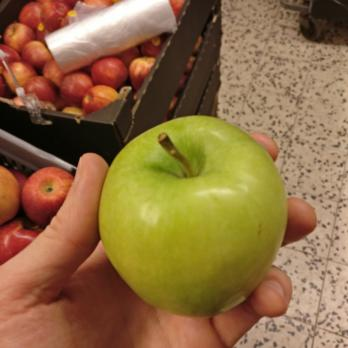
\includegraphics[height=1cm]{Chapter2/tikz/Golden-Delicious_031.jpg}};}},
}

\begin{tikzpicture}
	%\node at (0.5,-1){\begin{tabular}{c}input image\\layer $l = 0$\end{tabular}};
	\node at (0.5,2){\begin{tabular}{l}{\sf Inputs} \end{tabular}};
	\node at (2.,2){\begin{tabular}{l}{\sf Conv1} \end{tabular}};
	\node at (4.25,2){\begin{tabular}{l}{\sf Pooling1} \end{tabular}};
	\node at (6.2,2){\begin{tabular}{l}{\sf Conv2} \end{tabular}};
	\node at (8.8,2){\begin{tabular}{l}{\sf Pooling2} \end{tabular}};
	\node at (11.25,2){\begin{tabular}{l}{\sf FC} \end{tabular}};
	\node at (13.25,2){\begin{tabular}{l}{\sf Outputs} \end{tabular}};
	
	%\draw (0,0) -- (1,0) -- (1,1) -- (0,1) -- (0,0);
	\draw [path image,draw=black, thick] (0,0) rectangle (1,1);
	
	%\node at (3,3.5){\begin{tabular}{c}convolutional layer\\with non-linearities\\layer $l = 1$\end{tabular}};
	
	%\draw[fill=black,opacity=0.8,draw=black] (2.75,1.25) -- (3.75,1.25) -- (3.75,2.25) -- (2.75,2.25) -- (2.75,1.25);
	%\draw[fill=black,opacity=0.8,draw=black] (2.5,1) -- (3.5,1) -- (3.5,2) -- (2.5,2) -- (2.5,1);
	%\draw[fill=black,opacity=0.8,draw=black] (2.25,0.75) -- (3.25,0.75) -- (3.25,1.75) -- (2.25,1.75) -- (2.25,0.75);
	%\draw[fill=black,opacity=0.8,draw=black] (2,0.5) -- (3,0.5) -- (3,1.5) -- (2,1.5) -- (2,0.5);
	%\draw[fill=black,opacity=0.8,draw=black] (1.75,0.25) -- (2.75,0.25) -- (2.75,1.25) -- (1.75,1.25) -- (1.75,0.25);
	
	\draw[fill=black!50,opacity=0.8,draw=black] (2.0,0.5) -- (3.0,0.5) -- (3.0,1.5) -- (2.0,1.5) -- (2.0,0.5);
	\draw[fill=black!10,opacity=0.8,draw=black] (1.9,0.4) -- (2.9,0.4) -- (2.9,1.4) -- (1.9,1.4) -- (1.9,0.4);
	\draw[fill=black!50,opacity=0.8,draw=black] (1.8,0.3) -- (2.8,0.3) -- (2.8,1.3) -- (1.8,1.3) -- (1.8,0.3);
	\draw[fill=black!10,opacity=0.8,draw=black] (1.7,0.2) -- (2.7,0.2) -- (2.7,1.2) -- (1.7,1.2) -- (1.7,0.2);
	\draw[fill=black!50,opacity=0.8,draw=black] (1.6,0.1) -- (2.6,0.1) -- (2.6,1.1) -- (1.6,1.1) -- (1.6,0.1);
	\draw[fill=black!10,opacity=0.8,draw=black] (1.5,0) -- (2.5,0) -- (2.5,1) -- (1.5,1) -- (1.5,0);
	% conv box
	\draw (0.6,0.5) -- (0.8,0.5) -- (0.8,0.7) -- (0.6,0.7) -- (0.6,0.5);
	
	\draw (0.8,0.5) -- (2.2,0.6);
	\draw (0.8,0.7) -- (2.2,0.6);
	
	%\node at (4.5,-1){\begin{tabular}{c}subsampling layer\\layer $l = 3$\end{tabular}};
	
	%\draw[fill=black,opacity=0.8,draw=black] (5,1.25) -- (5.75,1.25) -- (5.75,2) -- (5,2) -- (5,1.25);
	%\draw[fill=black,opacity=0.8,draw=black] (4.75,1) -- (5.5,1) -- (5.5,1.75) -- (4.75,1.75) -- (4.75,1);
	%\draw[fill=black,opacity=0.8,draw=black] (4.5,0.75) -- (5.25,0.75) -- (5.25,1.5) -- (4.5,1.5) -- (4.5,0.75);
	%\draw[fill=black,opacity=0.8,draw=black] (4.25,0.5) -- (5,0.5) -- (5,1.25) -- (4.25,1.25) -- (4.25,0.5);
	%\draw[fill=black,opacity=0.8,draw=black] (4,0.25) -- (4.75,0.25) -- (4.75,1) -- (4,1) -- (4,0.25);
	%\draw[fill=black,opacity=0.8,draw=black] (3.75,0) -- (4.5,0) -- (4.5,0.75) -- (3.75,0.75) -- (3.75,0);
	
	\draw[fill=black!50,opacity=0.8,draw=black] (4.25,0.5) -- (5.0,0.5) -- (5.0,1.25) -- (4.25,1.25) -- (4.25,0.5);
	\draw[fill=black!10,opacity=0.8,draw=black] (4.15,0.4) -- (4.9,0.4) -- (4.9,1.15) -- (4.15,1.15) -- (4.15,0.4);
	\draw[fill=black!50,opacity=0.8,draw=black] (4.05,0.3) -- (4.8,0.3) -- (4.8,1.05) -- (4.05,1.05) -- (4.05,0.3);
	\draw[fill=black!10,opacity=0.8,draw=black] (3.95,0.2) -- (4.7,0.2) -- (4.7,0.95) -- (3.95,0.95) -- (3.95,0.2);
	\draw[fill=black!50,opacity=0.8,draw=black] (3.85,0.1) -- (4.6,0.1) -- (4.6,0.85) -- (3.85,0.85) -- (3.85,0.1);
	\draw[fill=black!10,opacity=0.8,draw=black] (3.75,0) -- (4.5,0) -- (4.5,0.75) -- (3.75,0.75) -- (3.75,0);
	
	% pooling box
	\draw (1.6,0.1) -- (1.8,0.1) -- (1.8,0.3) -- (1.6,0.3) -- (1.6,0.1);
	
	\draw (1.8,0.1) -- (3.9,0.15);
	\draw (1.8,0.3) -- (3.9,0.15);
	
	%\node at (7,3.5){\begin{tabular}{c}convolutional layer\\with non-linearities\\layer $l = 4$\end{tabular}};
	
	%\draw[fill=black,opacity=0.8,draw=black] (7.5,1.75) -- (8.25,1.75) -- (8.25,2.5) -- (7.5,2.5) -- (7.5,1.75);
	%\draw[fill=black,opacity=0.8,draw=black] (7.25,1.5) -- (8,1.5) -- (8,2.25) -- (7.25,2.25) -- (7.25,1.5);
	%\draw[fill=black,opacity=0.8,draw=black] (7,1.25) -- (7.75,1.25) -- (7.75,2) -- (7,2) -- (7,1.25);
	%\draw[fill=black,opacity=0.8,draw=black] (6.75,1) -- (7.5,1) -- (7.5,1.75) -- (6.75,1.75) -- (6.75,1);
	%\draw[fill=black,opacity=0.8,draw=black] (6.5,0.75) -- (7.25,0.75) -- (7.25,1.5) -- (6.5,1.5) -- (6.5,0.75);
	%\draw[fill=black,opacity=0.8,draw=black] (6.25,0.5) -- (7,0.5) -- (7,1.25) -- (6.25,1.25) -- (6.25,0.5);
	%\draw[fill=black,opacity=0.8,draw=black] (6,0.25) -- (6.75,0.25) -- (6.75,1) -- (6,1) -- (6,0.25);
	%\draw[fill=black,opacity=0.8,draw=black] (5.75,0) -- (6.5,0) -- (6.5,0.75) -- (5.75,0.75) -- (5.75,0);
	
	\draw[fill=black!50,opacity=0.8,draw=black] (6.65,0.9) -- (7.4,0.9) -- (7.4,1.65) -- (6.65,1.65) -- (6.65,0.9);			
	\draw[fill=black!10,opacity=0.8,draw=black] (6.55,0.8) -- (7.3,0.8) -- (7.3,1.55) -- (6.55,1.55) -- (6.55,0.8);			
	\draw[fill=black!50,opacity=0.8,draw=black] (6.45,0.7) -- (7.2,0.7) -- (7.2,1.45) -- (6.45,1.45) -- (6.45,0.7);	
	\draw[fill=black!10,opacity=0.8,draw=black] (6.35,0.6) -- (7.1,0.6) -- (7.1,1.35) -- (6.35,1.35) -- (6.35,0.6);		
	\draw[fill=black!50,opacity=0.8,draw=black] (6.25,0.5) -- (7.0,0.5) -- (7.0,1.25) -- (6.25,1.25) -- (6.25,0.5);
	\draw[fill=black!10,opacity=0.8,draw=black] (6.15,0.4) -- (6.9,0.4) -- (6.9,1.15) -- (6.15,1.15) -- (6.15,0.4);
	\draw[fill=black!50,opacity=0.8,draw=black] (6.05,0.3) -- (6.8,0.3) -- (6.8,1.05) -- (6.05,1.05) -- (6.05,0.3);
	\draw[fill=black!10,opacity=0.8,draw=black] (5.95,0.2) -- (6.7,0.2) -- (6.7,0.95) -- (5.95,0.95) -- (5.95,0.2);
	\draw[fill=black!50,opacity=0.8,draw=black] (5.85,0.1) -- (6.6,0.1) -- (6.6,0.85) -- (5.85,0.85) -- (5.85,0.1);
	\draw[fill=black!10,opacity=0.8,draw=black] (5.75,0) -- (6.5,0) -- (6.5,0.75) -- (5.75,0.75) -- (5.75,0);
	
	% conv box
	\draw (3.95,0.45) -- (4.15,0.45) -- (4.15,0.65) -- (3.95,0.65) -- (3.95,0.45);
	
	\draw (4.15,0.45) -- (6.05,0.55);
	\draw (4.15,0.65) -- (6.05,0.55);
	
	%\node at (9.5,-1){\begin{tabular}{c}subsampling layer\\layer $l = 6$\end{tabular}};
	
	%\draw[fill=black,opacity=0.8,draw=black] (10,1.75) -- (10.5,1.75) -- (10.5,2.25) -- (10,2.25) -- (10,1.75);
	%\draw[fill=black,opacity=0.8,draw=black] (9.75,1.5) -- (10.25,1.5) -- (10.25,2) -- (9.75,2) -- (9.75,1.5);
	%\draw[fill=black,opacity=0.8,draw=black] (9.5,1.25) -- (10,1.25) -- (10,1.75) -- (9.5,1.75) -- (9.5,1.25);
	%\draw[fill=black,opacity=0.8,draw=black] (9.25,1) -- (9.75,1) -- (9.75,1.5) -- (9.25,1.5) -- (9.25,1);
	%\draw[fill=black,opacity=0.8,draw=black] (9,0.75) -- (9.5,0.75) -- (9.5,1.25) -- (9,1.25) -- (9,0.75);
	%\draw[fill=black,opacity=0.8,draw=black] (8.75,0.5) -- (9.25,0.5) -- (9.25,1) -- (8.75,1) -- (8.75,0.5);
	%\draw[fill=black,opacity=0.8,draw=black] (8.5,0.25) -- (9,0.25) -- (9,0.75) -- (8.5,0.75) -- (8.5,0.25);
	%\draw[fill=black,opacity=0.8,draw=black] (8.25,0) -- (8.75,0) -- (8.75,0.5) -- (8.25,0.5) -- (8.25,0);
	\draw[fill=black!50,opacity=0.8,draw=black] (9.15,0.9) -- (9.65,0.9) -- (9.65,1.4) -- (9.15,1.4) -- (9.15,0.9);
	\draw[fill=black!10,opacity=0.8,draw=black] (9.05,0.8) -- (9.55,0.8) -- (9.55,1.3) -- (9.05,1.3) -- (9.05,0.8);
	\draw[fill=black!50,opacity=0.8,draw=black] (8.95,0.7) -- (9.45,0.7) -- (9.45,1.2) -- (8.95,1.2) -- (8.95,0.7);
	\draw[fill=black!10,opacity=0.8,draw=black] (8.85,0.6) -- (9.35,0.6) -- (9.35,1.1) -- (8.85,1.1) -- (8.85,0.6);
	\draw[fill=black!50,opacity=0.8,draw=black] (8.75,0.5) -- (9.25,0.5) -- (9.25,1.0) -- (8.75,1.0) -- (8.75,0.5);
	\draw[fill=black!10,opacity=0.8,draw=black] (8.65,0.4) -- (9.15,0.4) -- (9.15,0.9) -- (8.65,0.9) -- (8.65,0.4);
	\draw[fill=black!50,opacity=0.8,draw=black] (8.55,0.3) -- (9.05,0.3) -- (9.05,0.8) -- (8.55,0.8) -- (8.55,0.3);
	\draw[fill=black!10,opacity=0.8,draw=black] (8.45,0.2) -- (8.95,0.2) -- (8.95,0.7) -- (8.45,0.7) -- (8.45,0.2);
	\draw[fill=black!50,opacity=0.8,draw=black] (8.35,0.1) -- (8.85,0.1) -- (8.85,0.6) -- (8.35,0.6) -- (8.35,0.1);
	\draw[fill=black!10,opacity=0.8,draw=black] (8.25,0) -- (8.75,0) -- (8.75,0.5) -- (8.25,0.5) -- (8.25,0);
	
	% pooling box
	\draw (6.2,0.1) -- (6.4,0.1) -- (6.4,0.3) -- (6.2,0.3) -- (6.2,0.1);
	
	\draw(6.4,0.1) -- (8.65,0.15);
	\draw (6.4,0.3) -- (8.65,0.15);
	
	%\node at (12,3.5){\begin{tabular}{c}fully connected layer\\layer $l = 7$\end{tabular}};
	
	%\draw[fill=black,draw=black,opacity=0.5] (10.5,0) -- (11,0) -- (12.5,1.75) -- (12,1.75) -- (10.5,0);
	\draw[fill=black!10,draw=black,opacity=0.8] (10.5,0.1) -- (11,0.1) -- (11.8,1.0) -- (11.3,1.) -- (10.5,0.1);
	
	% flatten lines
	\draw(8.75,0.0) -- (10.5,0.1);
	\draw(9.65,1.4) -- (11.3,1.0);
	%\draw (6.4,0.3) -- (8.65,0.15);
	
	%\node at (13,-1){\begin{tabular}{c}fully connected layer\\output layer $l = 8$\end{tabular}};
	
	\draw[fill=black!10,draw=black,opacity=0.8] (12.5,0.0) -- (13,0.0) -- (13.45,0.6) -- (12.95,0.6) -- (12.5,0.0);
	
	% fc lines
	\draw(11.0,0.1) -- (12.5,0.0);
	\draw(11.8,1.0) -- (12.95,0.6);
\end{tikzpicture}
	}
	\caption{Simple CNN architecture with two convolutional layers (Conv) for extracting feature maps, two subsampling layers performing a pooling operation (Pooling), and one fully-connected layer (FC) to produce the network output.}
	\label{fig:cnn_simple}
\end{figure}

\vspace{-3mm}
\paragraph{Convolutional Neural Networks.} 
Convolutional layers consist of a set of filters defined by adaptable parameters to capture relationships between neighboring features in the data~\cite{lecun1998gradient}. %Convolutional layers consist of a set of filters with adaptable parameters to capture relationships between neighboring features in the data~\cite{lecun1998gradient}. 
Extracting the feature representations from one layer corresponds to convolving the input data with all filters, where the parameters in each filter are shared across every spatial location of the input. 
%Corresponding to convolving the data with a filter defined by these parameters
%The parameters in every filter are shared across every spatial location in the data when extracting the succeeding feature representation. 
This design choice enables each filter to extract important features at any position in the data. Furthermore, parameter sharing also reduces the amount of parameters in the network and lowers the number of operations for computing the outputs. Figure \ref{fig:cnn_simple} shows an illustration of a CNN architecture. Each filter slides across the width and height of the input to compute dot products between the filter weights and the local input region to produce a 2-dimensional feature map. The feature maps from all filters are then stacked depth-wise to obtain the output volume, which are often subsampled along their spatial dimensions with a pooling operation after a non-linear activation function. The feature maps in the last subsampling layer are flattened and fed into an arbitrary number of fully-connected layers (an MLP) to produce the final output. 


\vspace{-3mm}
\begin{wrapfigure}{r}{0.39\textwidth}
	\centering
	\vspace{-3mm}
	\resizebox{0.39\textwidth}{!}{
		
    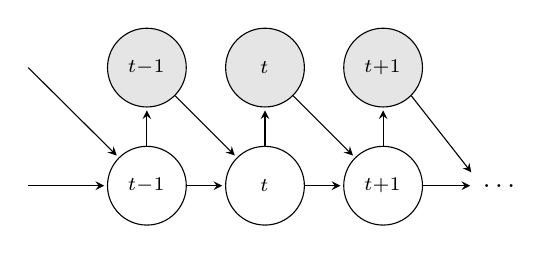
\begin{tikzpicture}[shorten >=1pt]
	\tikzstyle{unit}=[draw,shape=circle,minimum size=1.0cm]
	%\tikzstyle{box}=[draw,shape=rectangle,minimum size=1.0cm,rounded corners]
	
	\node[unit,fill=black!10](xtm1) at (0,1.5){$\vx_{t-1}$};
	\node[unit,fill=black!10](xt) at (1.5,1.5){$\vx_{t}$};
	\node[unit,fill=black!10](xtp1) at (3.0,1.5){$\vx_{t+1}$};
	
	\node[unit,fill=white](htm1) at (0,0){$\vh_{t-1}$};
	\node[unit,fill=white](ht) at (1.5,0){$\vh_{t}$};
	\node[unit,fill=white](htp1) at (3.0,0){$\vh_{t+1}$};
	
	\node (dots) at (4.5,0){\dots};
	
	\draw[-stealth] ([xshift=-1.0cm]xtm1.west) -> (htm1.north west); 
	\draw[-stealth] ([xshift=-1.0cm]htm1.west) -> (htm1.west); 
	
	\draw[-stealth] (htm1.north) -> (xtm1.south); 
	\draw[-stealth] (ht.north) -> (xt.south); 
	\draw[-stealth] (htp1.north) -> (xtp1.south); 
	
	\draw[-stealth] (htm1.east) -> (ht.west); 
	\draw[-stealth] (ht.east) -> (htp1.west); 
	\draw[-stealth] (htp1.east) -> (dots.west); 
	
	\draw[-stealth] (xtm1.south east) -> (ht.north west);
	\draw[-stealth] (xt.south east) -> (htp1.north west);
	\draw[-stealth] (xtp1.south east) -> (dots.north west);
	
\end{tikzpicture}
	}
	\captionsetup{width=.95\linewidth}
	\caption{Graphical representation of RNN.}
	\vspace{-3mm}
	\label{fig:rnn}
\end{wrapfigure}
\paragraph{Recurrent Neural Networks.} RNNs are a family of neural network models specialized for processing sequences of data. These networks predicts the next output given the past sequence and uses an extension of backpropagation to compute gradients across different time steps. 
Similar to CNNs, RNNs apply parameter sharing across time steps to enable extracting relevant information that can appear at different positions in the sequence. RNNs makes an assumption that all relevant information about the past sequence $\vx_{1:t-1}$ can be summarized in a hidden state $\vh_t$. The state evolves over time through the updated equation $\vh_t = f_{\vtheta}(\vh_{t-1}, \vx_{t-1})$ where $f_{\vtheta}$ is a neural network for capturing the long-term dependencies. Common choices for this network are the Long Short-Term Memory (LSTM)~\cite{hochreiter1997long} and Gated Recurrent Unit (GRU)~\cite{chung2014empirical} which use gating functions for determining what information is relevant for the future time steps. Figure \ref{fig:rnn} shows a graphical representation of an RNN. The initial hidden state $\vh_0$ is usually set to zero or learned. 

\vspace{3mm}
\noindent Attention-based network architectures, such as Transformers~\cite{vaswani2017attention, dosovitskiy2020image} and Graph Neural Networks~\cite{battaglia2018relational, zhou2020graph}, are not covered in this thesis; we refer the reader to the provided references for information on these networks.



\subsection{Deep Autoencoders}\label{sec:deep_autoencoders}

\begin{wrapfigure}{r}{0.42\textwidth}
	\centering
	\vspace{-3mm}
	\resizebox{0.39\textwidth}{!}{
		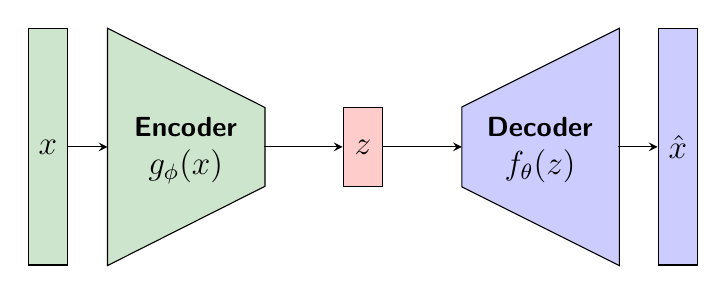
\begin{tikzpicture}
	%\node at (0.0,2.0){\begin{tabular}{c}{\sf Inputs} \end{tabular}};
	%\node at (8.0,2.0){\begin{tabular}{c}{\sf Reconstructed \\ \sf Inputs} \end{tabular}};
	
	\node[fill=Green!20, minimum width=0.5cm, minimum height=3.0cm, draw] (x) at (0,0) {\large $\boldsymbol x$};
	
	\draw[fill=Green!20] ([xshift=0.5cm]x.north east) -- ([xshift=2.5cm,yshift=0.5cm]x.east) -- ([xshift=2.5cm,yshift=-0.5cm]x.east) -- ([xshift=0.5cm]x.south east) -- cycle; 
	\node at (1.75,0.25) {{\sf \textbf{Encoder}}};
	\node at (1.75,-0.25) {\large $g_{\boldsymbol{\phi}}(\boldsymbol{x})$};
	
	\node[fill=red!20, minimum width=0.5cm, minimum height=1.0cm, draw] (z) at (4.0cm,0.0) {\large $\boldsymbol z$};
	
	\draw[fill=blue!20] ([xshift=1.0cm]z.north east) -- ([xshift=3.0cm,yshift=1.0cm]z.north east) -- ([xshift=3.0cm,yshift=-1.0cm]z.south east) -- ([xshift=1.0cm]z.south east) -- cycle;
	\node at (6.25,0.25) {{\sf \textbf{Decoder}}};
	\node at (6.25,-0.25) {\large $f_{\boldsymbol{\theta}}(\boldsymbol{z})$};
	
	\node[fill=blue!20, minimum width=0.5cm, minimum height=3.0cm, draw] (xhat) at (8.0cm,0) {\large $\boldsymbol{\hat{x}}$};
	
	\draw[-stealth] (x.east) -> ([xshift=0.5cm]x.east);
	\draw[-stealth] ([xshift=-1.0cm]z.west) -> (z.west);
	\draw[-stealth] (z.east) -> ([xshift=1.0cm]z.east);
	\draw[-stealth] ([xshift=-0.5cm]xhat.west) -> (xhat.west);
\end{tikzpicture}
	}
	\captionsetup{width=.95\linewidth}
	\caption{Illustration of an autoencoder network.}
	\label{fig:autoencoder}
	\vspace{-3mm}
\end{wrapfigure}
A common network architecture for learning latent representations of high-dimensional data in unsupervised fashions with deep learning are autoencoders. These architectures are typically built using two networks called decoder $f_{\vtheta}$ and encoder $g_{\vphi}$ with a bottleneck layer between the networks that extracts a low-dimensional representation $\vz$ of the data $\vx$. The idea is that the learned representation $\vz$ should contain enough relevant information for reconstructing the input data. Figure \ref{fig:autoencoder} shows an illustration of an autoencoder network. The encoder extracts the latent representation with $\vz = g_{\vphi}(\vx)$, while the decoder aims to reconstruct the original input, such that $\hat{\vx} = f_{\vtheta}(\vz)$ where $\hat{\vx} \approx \vx$. There exist various autoencoder approaches for improving the quality of the learned representations. For example, denoising autoencoders~\cite{vincent2008extracting} adds noise to the input data to avoid overfitting, and sparse autoencoders~\cite{ng2011sparse} induces adds sparsity constraints on the activation functions to improve robustness.



\begin{comment}

\begin{figure}[t]
	\centering
	\resizebox{0.6\textwidth}{!}{
		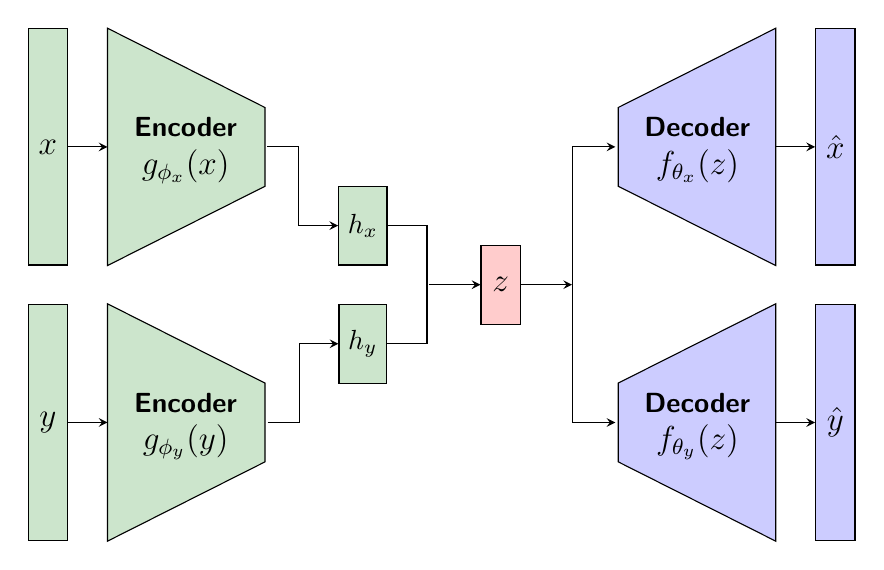
\begin{tikzpicture}
	
	\node[fill=Green!20, minimum width=0.5cm, minimum height=3.0cm, draw] (y) at (0,0) {\large $\boldsymbol y$};
	
	\node[fill=Green!20, minimum width=0.5cm, minimum height=3.0cm, draw] (x) at (0,3.5) {\large $\boldsymbol x$};
	
	\draw[fill=Green!20] ([xshift=0.5cm]x.north east) -- ([xshift=2.5cm,yshift=0.5cm]x.east) -- ([xshift=2.5cm,yshift=-0.5cm]x.east) -- ([xshift=0.5cm]x.south east) -- cycle; 
	\node at (1.75,3.75) {{\sf \textbf{Encoder}}};
	\node at (1.75,3.25) {\large $g_{\boldsymbol{\phi_x}}(\boldsymbol{x})$};
	
	
	\draw[fill=Green!20] ([xshift=0.5cm]y.north east) -- ([xshift=2.5cm,yshift=0.5cm]y.east) -- ([xshift=2.5cm,yshift=-0.5cm]y.east) -- ([xshift=0.5cm]y.south east) -- cycle; 
	\node at (1.75,0.25) {{\sf \textbf{Encoder}}};
	\node at (1.75,-0.25) {\large $g_{\boldsymbol{\phi_y}}(\boldsymbol{y})$};
	
	
	\node[fill=Green!20, minimum width=0.6cm, minimum height=1.0cm, draw] (hx) at (4.0cm,2.5cm) { $\boldsymbol{h_x}$};
	\node[fill=Green!20, minimum width=0.6cm, minimum height=1.0cm, draw] (hy) at (4.0cm,1.0cm) { $\boldsymbol{h_y}$};
	
	\node[fill=red!20, minimum width=0.5cm, minimum height=1.0cm, draw] (z) at (5.75cm,1.75cm) {\large $\boldsymbol z$};
	
	\draw[-stealth] ([xshift=-0.9cm,yshift=1.0cm]hx.west) -- ([xshift=-0.5cm,yshift=1.0cm]hx.west) |- ([xshift=-0.5cm]hx.west) -> (hx.west);
	\draw[-stealth] ([xshift=-0.9cm,yshift=-1.0cm]hy.west) -- ([xshift=-0.5cm,yshift=-1.0cm]hy.west) |- ([xshift=-0.5cm]hy.west) -> (hy.west);
	\draw (hx.east) -- ([xshift=0.5cm]hx.east) |- ([xshift=0.5cm]hy.east) -- (hy.east);
	\draw[-stealth] ([xshift=-0.65cm]z.west) -> (z.west);
	
	
	\node[fill=blue!20, minimum width=0.5cm, minimum height=3.0cm, draw] (xhat) at (10cm,3.5) {\large $\boldsymbol{\hat{x}}$};
	
	\draw[fill=blue!20] ([xshift=-0.5cm]xhat.north west) -- ([xshift=-2.5cm,yshift=0.5cm]xhat.west) -- ([xshift=-2.5cm,yshift=-0.5cm]xhat.west) -- ([xshift=-0.5cm]xhat.south west) -- cycle; 
	\node at (8.25,3.75) {{\sf \textbf{Decoder}}};
	\node at (8.25,3.25) {\large $f_{\boldsymbol{\theta_x}}(\boldsymbol{z})$};
	
	\node[fill=blue!20, minimum width=0.5cm, minimum height=3.0cm, draw] (yhat) at (10cm,0) {\large $\boldsymbol{\hat{y}}$};
	
	\draw[fill=blue!20] ([xshift=-0.5cm]yhat.north west) -- ([xshift=-2.5cm,yshift=0.5cm]yhat.west) -- ([xshift=-2.5cm,yshift=-0.5cm]yhat.west) -- ([xshift=-0.5cm]yhat.south west) -- cycle; 
	\node at (8.25,0.25) {{\sf \textbf{Decoder}}};
	\node at (8.25,-0.25) {\large $f_{\boldsymbol{\theta_y}}(\boldsymbol{z})$};
	
	\draw[-stealth] (z.east) -> ([xshift=0.65cm]z.east);
	\draw[-stealth] ([xshift=0.65cm]z.east) -- ([xshift=0.65cm,yshift=1.75cm]z.east) -> ([xshift=1.2cm,yshift=1.75cm]z.east);
	\draw[-stealth] ([xshift=0.65cm]z.east) -- ([xshift=0.65cm,yshift=-1.75cm]z.east) -> ([xshift=1.2cm,yshift=-1.75cm]z.east);
	
	\draw[-stealth] ([xshift=-0.5cm]xhat.west) -- (xhat.west);
	\draw[-stealth] ([xshift=-0.5cm]yhat.west) -- (yhat.west);
	
	\draw[-stealth] (x.east) -- ([xshift=0.5cm]x.east);
	\draw[-stealth] (y.east) -- ([xshift=0.5cm]y.east);
	
	
\end{tikzpicture}
	}
	\caption{Illustration of multimodal autoencoder network for learning joint representation $\vz$ from the different but related data types $\vx$ and $\vy$. The joint representation $\vz$ is obtained by combining the intermediate representations $\vh_{\vx}$ and $\vh_{\vy}$. %Illustration of multimodal autoencoder network for learning joint representation $\vz$ from the different but related data types $\vx$ and $\vy$. 
	}
	\label{fig:multimodal_autoencoder1}
	\vspace{-3mm}
\end{figure}
\end{comment}

\begin{wrapfigure}{r}{0.59\textwidth}
	\centering
	%\vspace{-3mm}
	\resizebox{0.54\textwidth}{!}{
		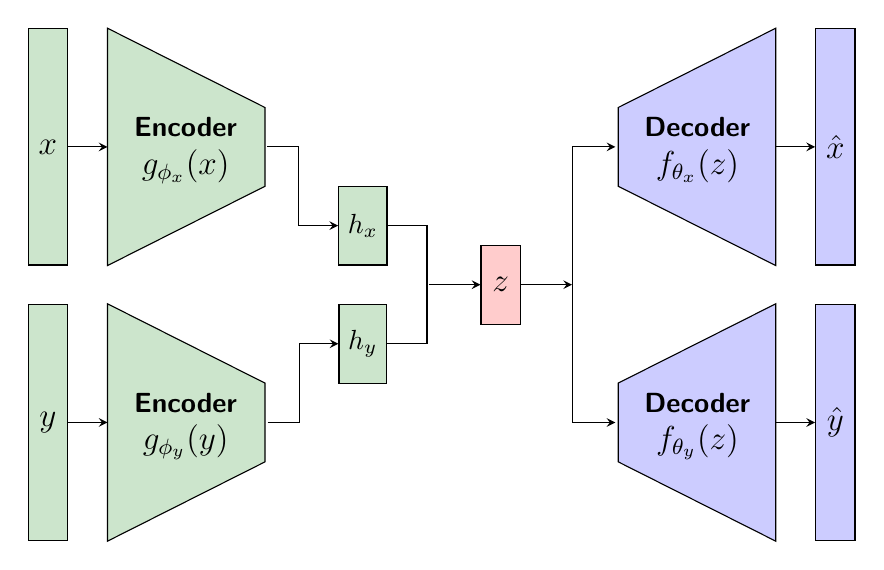
\begin{tikzpicture}
	
	\node[fill=Green!20, minimum width=0.5cm, minimum height=3.0cm, draw] (y) at (0,0) {\large $\boldsymbol y$};
	
	\node[fill=Green!20, minimum width=0.5cm, minimum height=3.0cm, draw] (x) at (0,3.5) {\large $\boldsymbol x$};
	
	\draw[fill=Green!20] ([xshift=0.5cm]x.north east) -- ([xshift=2.5cm,yshift=0.5cm]x.east) -- ([xshift=2.5cm,yshift=-0.5cm]x.east) -- ([xshift=0.5cm]x.south east) -- cycle; 
	\node at (1.75,3.75) {{\sf \textbf{Encoder}}};
	\node at (1.75,3.25) {\large $g_{\boldsymbol{\phi_x}}(\boldsymbol{x})$};
	
	
	\draw[fill=Green!20] ([xshift=0.5cm]y.north east) -- ([xshift=2.5cm,yshift=0.5cm]y.east) -- ([xshift=2.5cm,yshift=-0.5cm]y.east) -- ([xshift=0.5cm]y.south east) -- cycle; 
	\node at (1.75,0.25) {{\sf \textbf{Encoder}}};
	\node at (1.75,-0.25) {\large $g_{\boldsymbol{\phi_y}}(\boldsymbol{y})$};
	
	
	\node[fill=Green!20, minimum width=0.6cm, minimum height=1.0cm, draw] (hx) at (4.0cm,2.5cm) { $\boldsymbol{h_x}$};
	\node[fill=Green!20, minimum width=0.6cm, minimum height=1.0cm, draw] (hy) at (4.0cm,1.0cm) { $\boldsymbol{h_y}$};
	
	\node[fill=red!20, minimum width=0.5cm, minimum height=1.0cm, draw] (z) at (5.75cm,1.75cm) {\large $\boldsymbol z$};
	
	\draw[-stealth] ([xshift=-0.9cm,yshift=1.0cm]hx.west) -- ([xshift=-0.5cm,yshift=1.0cm]hx.west) |- ([xshift=-0.5cm]hx.west) -> (hx.west);
	\draw[-stealth] ([xshift=-0.9cm,yshift=-1.0cm]hy.west) -- ([xshift=-0.5cm,yshift=-1.0cm]hy.west) |- ([xshift=-0.5cm]hy.west) -> (hy.west);
	\draw (hx.east) -- ([xshift=0.5cm]hx.east) |- ([xshift=0.5cm]hy.east) -- (hy.east);
	\draw[-stealth] ([xshift=-0.65cm]z.west) -> (z.west);
	
	
	\node[fill=blue!20, minimum width=0.5cm, minimum height=3.0cm, draw] (xhat) at (10cm,3.5) {\large $\boldsymbol{\hat{x}}$};
	
	\draw[fill=blue!20] ([xshift=-0.5cm]xhat.north west) -- ([xshift=-2.5cm,yshift=0.5cm]xhat.west) -- ([xshift=-2.5cm,yshift=-0.5cm]xhat.west) -- ([xshift=-0.5cm]xhat.south west) -- cycle; 
	\node at (8.25,3.75) {{\sf \textbf{Decoder}}};
	\node at (8.25,3.25) {\large $f_{\boldsymbol{\theta_x}}(\boldsymbol{z})$};
	
	\node[fill=blue!20, minimum width=0.5cm, minimum height=3.0cm, draw] (yhat) at (10cm,0) {\large $\boldsymbol{\hat{y}}$};
	
	\draw[fill=blue!20] ([xshift=-0.5cm]yhat.north west) -- ([xshift=-2.5cm,yshift=0.5cm]yhat.west) -- ([xshift=-2.5cm,yshift=-0.5cm]yhat.west) -- ([xshift=-0.5cm]yhat.south west) -- cycle; 
	\node at (8.25,0.25) {{\sf \textbf{Decoder}}};
	\node at (8.25,-0.25) {\large $f_{\boldsymbol{\theta_y}}(\boldsymbol{z})$};
	
	\draw[-stealth] (z.east) -> ([xshift=0.65cm]z.east);
	\draw[-stealth] ([xshift=0.65cm]z.east) -- ([xshift=0.65cm,yshift=1.75cm]z.east) -> ([xshift=1.2cm,yshift=1.75cm]z.east);
	\draw[-stealth] ([xshift=0.65cm]z.east) -- ([xshift=0.65cm,yshift=-1.75cm]z.east) -> ([xshift=1.2cm,yshift=-1.75cm]z.east);
	
	\draw[-stealth] ([xshift=-0.5cm]xhat.west) -- (xhat.west);
	\draw[-stealth] ([xshift=-0.5cm]yhat.west) -- (yhat.west);
	
	\draw[-stealth] (x.east) -- ([xshift=0.5cm]x.east);
	\draw[-stealth] (y.east) -- ([xshift=0.5cm]y.east);
	
	
\end{tikzpicture}
	}
	\captionsetup{width=.95\linewidth}
	\caption{Illustration of a multimodal autoencoder network for learning a joint representation $\vz$ from the different but related data types $\vx$ and $\vy$. The joint representation $\vz$ is obtained by combining the intermediate representations $\vh_{\vx}$ and $\vh_{\vy}$.
	}
	\label{fig:multimodal_autoencoder}
	\vspace{-3mm}
\end{wrapfigure}
\paragraph{Multimodal Autoencoders.} Autoencoders can easily be extended to handling multiple types of data. The goal here is usually to learn one joint latent representation for capturing correspondences between the data types~\cite{baltruvsaitis2018multimodal}. Consider the multimodal dataset $\gD = \{(\vx_i, \vy_i)\}_{i=1}^{N}$ where $\vx$ and $\vy$ originate from two different data views (real-world images, web images) or modalities (visual signals, text descriptions) that share some high-level information. For example, $\vx$ could be an image of a living room and $\vy$ is a text sentence describing the appearance of the room, where objects are located etc. 
Figure \ref{fig:multimodal_autoencoder} shows an illustration of the network architecture. The input $\vx$ and $\vy$ have two separate encoders, $g_{\vphi_{\vx}}(\vx)$ and $g_{\vphi_{\vy}}(\vy)$, that extracts the intermediate latent representations $\vh_{\vx}$ and $\vh_{\vy}$ respectively. The intermediate representations are then combined into the joint latent representation $\vz$, often through some element-wise operation (addition, multiplication) or concatenation. The joint multimodal representation $\vz$ is then passed through two separate decoder networks, $f_{\vtheta_{\vx}}(\vz)$ and $f_{\vtheta_{\vy}}(\vz)$, for predicting the original input data separately. 
Combining different modalities, such as images, natural language, and audio signals, with autoencoders for learning more rich representations of data has been studied frequently the last decade~\cite{baltruvsaitis2018multimodal,ngiam2011multimodal,wang2015deep,vedantam2017generative,wu2018multimodal,owens2018audio}
%Combining different modalities, such as image and video, natural language, and audio signals, with autoencoders for learning more rich representations of data has been studied frequently the last decade~\cite{owens2018audio, ngiam2011multimodal, silberer2014learning, lee2020making} [Add REFs]. 
One advantage is that the network architecture can be trained in an trained end-to-end fashion to be used for both learning representations and making predictions of the used data types.
However, a major challenge is how to handle scenarios where some data types could be missing. An option here is to learn a joint representation by using a single encoder for the data type that is available at both training and test phases that is used for predicting each data type~\cite{ngiam2011multimodal}. 
%We can also  handle missing modalities for the encoders which enables cross-modal data generation between the modalities.


%Learning representations from different types of data is a highly active research field in deep learning~\cite{baltruvsaitis2018multimodal}. Combining visual data with other modalities such as natural language and audio signals for learning more rich representations of data has been studied frequently the last decade~\cite{owens2018audio, ngiam2011multimodal, silberer2014learning, lee2020making} [Add REFs]. A common framework in such applications is to use autoencoders for incorporating information from the different data types into a single joint representation. Learning from multiple sources then opens up for capturing correspondences between the data types and obtaining better representations that can be used for downstream tasks such as classification. 

%Let $\vx$ and $\vy$ originate from two different data sources but share some high-level information. For example, $\vx$ could be an image of a living room and $\vy$ is text describing the appearance of the room, where objects are located etc. Constructing a joint representation is then done by projecting both $\vx$ and $\vy$ with separate encoder networks into the same latent space. The joint multimodal representation is then passed through two separate decoder networks used for predicting the original input data individually. The advantage of multimodal autoencoders is that they can be trained end-to-end for both learning representations as well as making predictions of the used modalities. However, a major challenge is how to handle scenarios where modalities might be missing. One option is to only encode the data modality that we know will be available at both training and test phases and then establish a joint representation by decoding two both modalities~\cite{ngiam2011multimodal}.

%Multimodal autoencoders have frequently been extended to deep generative models, mainly VAEs~\cite{wang2016deep, wu2018multimodal, shi2019variational, vedantam2017generative, suzuki2016joint}. These models are capable of generating new data through sampling from the latent space in addition to learning joint representations. Furthermore, they can handle missing modalities for the encoders which enables cross-modal data generation between the modalities. In Paper B [Add REF], we employ Variational Canonical Correlation Analysis (VCCA) for learning joint representations of natural images and web-scraped information of grocery items to facilitate learning image classifiers. 




%A common architecture type for deep learning in unsupervised learning are autoencoders for learning hidden representations of unlabeled data. Autoencoders are commonly used for dimensionality reduction of high-dimensional data, where the lower-dimensional representation can be used for classification tasks, or to visualize hidden structures in the data that are hard to reveal from the original input data. The objective of the model is to reconstruct the original input data. The network architecture is built using two networks called \textit{encoder} and \textit{decoder} with a bottleneck layer between the networks for extracting the hidden representation $\vh$. The encoder and decoder architectures can be of any neural network type, such as MLPs, CNNs, or RNNs, that fits the given dataset. The encoder is used for obtaining the hidden representation of the input data, while the decoder tries to reconstruct the original input from the obtained representation. Therefore, the idea is that the learned representation should contain the relevant information for reconstructing the data. 

%Mathematically, we denote the decoder as $f_{\vtheta}$ and the encoder as $g_{\vphi}$. The encoder extracts the hidden representation $\vh = g_{\vphi}(\vx)$ from the input $\vx$, then the decoder produces a reconstruction $\hat{\vx} = f_{\vtheta}(\vh)$ from $\vh$. We train the encoder and decoder simultaneously by minimizing a reconstruction loss $\gL(f_{\vtheta}(g_{\vphi}(\vx)), \vx)$, for instance mean-squared error loss, using SGD similarly as for the feedforward networks described above. There exist various kinds of methods for improving the quality of the learned representations in autoencoders. For example, we can adjust target task by adding noise to the inputs and let the decoder reconstruct the original input from noise variants~\cite{vincent2008extracting}, or we can induce different constraints in the bottleneck layer to, for example, obtain a sparse lower-dimensional representation of the data. Next, we will introduce the variational autoencoder which originates from latent variable models. 

\subsubsection{Variational Autoencoders}\label{sec:variational_autoencoders}

In this section, we give an overview of the variational autoencoder (VAE)~\cite{kingma2013auto, kingma2019introduction} that we apply for representation learning in Paper \ref{paperA} and \ref{paperB}. 
The VAE is a deep generative model that enable learning of data representations %learns representations of data 
by combining ideas from deep learning and probabilistic graphical models~\cite{koller2009probabilistic}. 
As commonly done in unsupervised learning, VAEs aim to learn a parametric distribution $p_{\vtheta}(\vx)$ that approximates the data distribution $p_{data}$ given a dataset $\gD = \{\vx^{(i)}\}_{i=1}^{N}$ where $\vx^{(i)} \sim p_{data}$. We frame the problem of learning $p_{\vtheta}(\vx)$ by expressing the distribution using latent variables $\vz$, such that
\begin{equation}\label{eq:px}
	p_{\vtheta}(\vx) = \int p_{\vtheta}(\vx, \vz) \, d\vz = \int p_{\vtheta}(\vx | \vz) p(\vz) \, d\vz,
\end{equation}
where the joint distribution $p_{\vtheta}(\vx, \vz)$ is the model which factorizes into the likelihood $p_{\vtheta}(\vx | \vz)$ and the prior distribution $p(\vz)$ for the latent variables. The latent variables $\vz$ are introduced for representing underlying structures and relationships in $\vx$ that can be difficult to observe from the data itself. We can view $\vz$ as containing meaningful information for the data generation process by assuming that the data was generated with the following steps: 
\begin{enumerate}[topsep=1pt,noitemsep]
	\item sample the latent vector $\vz \sim p(\vz)$ from the prior.
	\item generate data point $\vx \sim p_{\vtheta}(\vx | \vz)$ given the sampled $\vz$.
\end{enumerate}

\vspace{-3mm}
\paragraph{The Evidence Lower Bound.} The problem with learning the parameters $\vtheta$ that maximize $p_{\vtheta}(\vx)$ is that the integral in Equation \ref{eq:px} is almost always intractable due to the 
prohibitively large number of values for $\vz$ that need to be evaluated. %immense amount of values for $\vz$ that needs to be evaluated. 
Instead, we can reformulate the problem using Bayes' rule %compute $p_{\vtheta}(\vx)$ using Bayes' rule 
\begin{equation}
	p_{\vtheta}(\vx) = \frac{p_{\vtheta}(\vx | \vz) p(\vz) }{p_{\vtheta}(\vz | \vx)},
\end{equation}
where $p_{\vtheta}(\vz | \vx)$ is the posterior of $\vz$ given $\vx$ and $p_{\vtheta}(\vx | \vz)$ is the likelihood of $\vx$ given $\vz$. The posterior needs to be approximated using variational inference~\cite{zhang2018advances,blei2017variational}, where we define an approximate posterior distribution $q_{\vphi}(\vz | \vx)$ parameterized by $\vphi$ to infer the latents $\vz$.  
%where the posterior distribution $p_{\vtheta}(\vz | \vx)$ can facilitate faster learning by inferring the latents $\vz$ from data $\vx$. However, we need to resort to approximating the posterior using variational inference~\cite{zhang2018advances,blei2017variational} since the posterior needs access to $p_{\vtheta}(\vx)$ to be computed. We then define an approximate posterior distribution $q_{\vphi}(\vz | \vx)$ parameterized by $\vphi$ to infer the latents $\vz$. 
This allows us to form a lower bound on the marginal log-likelihood $\log p_{\vtheta}(\vx)$ given by 
\begin{align}\label{eq:elbo}
	\log p_{\vtheta}(\vx) \geq \E_{z \sim q_{\vphi}(\vz | \vx)}[\log p_{\vtheta}(\vx | \vz)] - \KL[q_{\vphi}(\vz |  \vx) \, || \, p(\vz)] ,
\end{align}
which is called the evidence lower bound (ELBO). The expected value over $\log p_{\vtheta}(\vx | \vz)$ can be estimated with Monte Carlo sampling using $q_{\vphi}(\vz | \vx)$, and the Kullback-Leibler (KL) divergence between $q_{\vphi}(\vz |  \vx)$ and $p(\vz)$ can be computed analytically depending on how we choose these distributions. Commonly, the approximate posterior is selected to be a Gaussian distribution $q_{\vphi}(\vz | \vx) = \gN(\vz; \vmu_{\vphi}(\vx), \text{diag}(\vsigma_{\vphi}(\vx)))$ where the parameters $\vphi$ are used for computing the mean $\vmu_{\vphi}(\vx)$ and standard deviation $\vsigma_{\vphi}(\vx)$ of the approximate posterior given $\vx$, and $\text{diag}(\cdot)$ is for constraining the covariance matrix to be a diagonal matrix. The prior distribution is also selected to be a zero-mean, standard Gaussian distribution $p(\vz) = \gN(\vz; \mathbf{0}, \mathbf{I})$ where $\mathbf{I}$ is the identity matrix. 

\begin{comment}
\begin{figure}[t]
	\centering
	\resizebox{0.6\textwidth}{!}{
		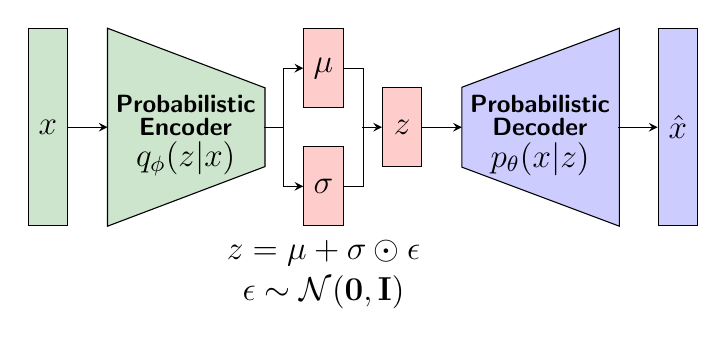
\begin{tikzpicture}
	
	
	\node[fill=Green!20, minimum width=0.5cm, minimum height=2.5cm, draw] (x) at (0,0) {\large $\boldsymbol x$};
	
	\draw[fill=Green!20] ([xshift=0.5cm]x.north east) -- ([xshift=2.5cm,yshift=0.5cm]x.east) -- ([xshift=2.5cm,yshift=-0.5cm]x.east) -- ([xshift=0.5cm]x.south east) -- cycle; 
	\node at (1.75,0.3) {{\small\sf \textbf{Probabilistic}}};
	\node at (1.75,0.0) {{\small\sf \textbf{Encoder}}};
	\node at (1.75,-0.4) {\large $q_{\boldsymbol{\phi}}(\boldsymbol{z} | \boldsymbol{x})$};
	
	\draw[-stealth] (x.east) -- ([xshift=0.5cm]x.east);
	
	\node[fill=red!20, minimum width=0.5cm, minimum height=1.0cm, draw] (mu) at (3.5cm,0.75cm) {\large $\boldsymbol{\mu}$};
	\node[fill=red!20, minimum width=0.5cm, minimum height=1.0cm, draw] (sigma) at (3.5cm,-0.75cm) {\large $\boldsymbol{\sigma}$};
	
	\node at (3.5cm,-1.6cm) {\large $\boldsymbol{z} = \boldsymbol{\mu} + \boldsymbol{\sigma} \odot \boldsymbol{\epsilon}$};
	\node at (3.5cm,-2.1cm) {\large $\boldsymbol{\epsilon} \sim \mathcal{N}(\mathbf{0}, \mathbf{I})$};
	\draw ([xshift=-0.5cm,yshift=-0.75cm]mu.west) -- ([xshift=-0.25cm,yshift=-0.75cm]mu.west);
	\draw[-stealth] ([xshift=-0.25cm,yshift=-0.75cm]mu.west) |- ([xshift=-0.25cm]mu.west) -- (mu.west);
	\draw[-stealth] ([xshift=-0.25cm,yshift=0.75cm]sigma.west) |- ([xshift=-0.25cm]sigma.west) -- (sigma.west);
	
	%\node[fill=red!20, minimum width=0.5cm, minimum height=1.0cm, draw] (z) at (5.0cm,0.0) {\large $\boldsymbol z$};
	\node[fill=red!20, minimum width=0.5cm, minimum height=1.0cm, draw] (z) at (4.5cm,0.0) {\large $\boldsymbol z$};
	\draw (mu.east) -- ([xshift=0.25cm]mu.east) |- ([xshift=-0.25cm]z.west);
	\draw (sigma.east) -- ([xshift=0.25cm]sigma.east) |- ([xshift=-0.25cm]z.west);
	\draw[-stealth] ([xshift=-0.25cm]z.west) -- (z.west);
	
	%\draw[-stealth] ([xshift=-2.5cm]z.west) -> ([xshift=-2.0cm]z.west);
	%\draw[-stealth] ([xshift=-0.5cm,yshift=-0.75cm]mu.west) -- ([xshift=-0.5cm]mu.west) |- (mu.west);
	%%%\draw[-stealth] ([xshift=-0.5cm,yshift=0.75cm]sigma.west) -- ([xshift=-0.5cm]sigma.west) |- (sigma.west);
	%%%\draw[-stealth] (mu.west) -- ([xshift=-0.5cm]mu.west) |- ([xshift=-0.5cm]sigma.west) -- (sigma.west);
	%\draw (mu.east) -- ([xshift=0.5cm]mu.east) |- ([xshift=0.5cm]sigma.east) -- (sigma.east);
	%\draw[-stealth] ([xshift=-0.45cm]z.west) -> (z.west);
	
	\draw[fill=blue!20] ([xshift=0.5cm]z.north east) -- ([xshift=2.5cm,yshift=0.75cm]z.north east) -- ([xshift=2.5cm,yshift=-0.75cm]z.south east) -- ([xshift=0.5cm]z.south east) -- cycle;
	\node at (6.25,0.3) {{\small\sf \textbf{Probabilistic}}};
	\node at (6.25,0.0) {{\small\sf \textbf{Decoder}}};
	\node at (6.25,-0.4) {\large $p_{\boldsymbol{\theta}}(\boldsymbol{x} | \boldsymbol{z})$};
	
	\node[fill=blue!20, minimum width=0.5cm, minimum height=2.5cm, draw] (xhat) at (8.0cm,0) {\large $\boldsymbol{\hat{x}}$};
	
	\draw[-stealth] (z.east) -- ([xshift=0.5cm]z.east);
	\draw[-stealth] ([xshift=-0.5cm]xhat.west) -- (xhat.west);
	
	
\end{tikzpicture}
	}
	\caption{Illustration of a VAE. 
	}
	\label{fig:vae1}
	\vspace{-3mm}
\end{figure}	
\end{comment}


\vspace{-3mm}
\begin{wrapfigure}{r}{0.48\textwidth}
	\centering
	\vspace{-2mm}
	\resizebox{0.45\textwidth}{!}{
		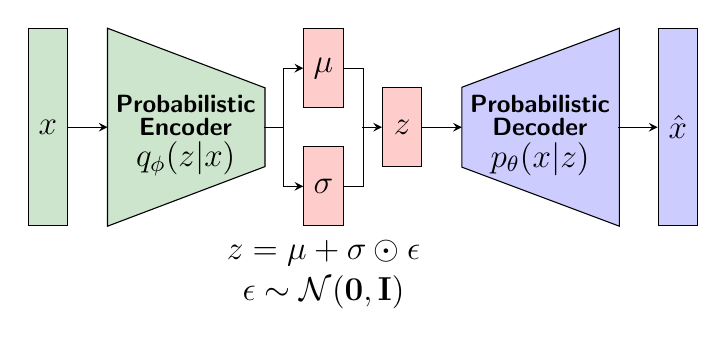
\begin{tikzpicture}
	
	
	\node[fill=Green!20, minimum width=0.5cm, minimum height=2.5cm, draw] (x) at (0,0) {\large $\boldsymbol x$};
	
	\draw[fill=Green!20] ([xshift=0.5cm]x.north east) -- ([xshift=2.5cm,yshift=0.5cm]x.east) -- ([xshift=2.5cm,yshift=-0.5cm]x.east) -- ([xshift=0.5cm]x.south east) -- cycle; 
	\node at (1.75,0.3) {{\small\sf \textbf{Probabilistic}}};
	\node at (1.75,0.0) {{\small\sf \textbf{Encoder}}};
	\node at (1.75,-0.4) {\large $q_{\boldsymbol{\phi}}(\boldsymbol{z} | \boldsymbol{x})$};
	
	\draw[-stealth] (x.east) -- ([xshift=0.5cm]x.east);
	
	\node[fill=red!20, minimum width=0.5cm, minimum height=1.0cm, draw] (mu) at (3.5cm,0.75cm) {\large $\boldsymbol{\mu}$};
	\node[fill=red!20, minimum width=0.5cm, minimum height=1.0cm, draw] (sigma) at (3.5cm,-0.75cm) {\large $\boldsymbol{\sigma}$};
	
	\node at (3.5cm,-1.6cm) {\large $\boldsymbol{z} = \boldsymbol{\mu} + \boldsymbol{\sigma} \odot \boldsymbol{\epsilon}$};
	\node at (3.5cm,-2.1cm) {\large $\boldsymbol{\epsilon} \sim \mathcal{N}(\mathbf{0}, \mathbf{I})$};
	\draw ([xshift=-0.5cm,yshift=-0.75cm]mu.west) -- ([xshift=-0.25cm,yshift=-0.75cm]mu.west);
	\draw[-stealth] ([xshift=-0.25cm,yshift=-0.75cm]mu.west) |- ([xshift=-0.25cm]mu.west) -- (mu.west);
	\draw[-stealth] ([xshift=-0.25cm,yshift=0.75cm]sigma.west) |- ([xshift=-0.25cm]sigma.west) -- (sigma.west);
	
	%\node[fill=red!20, minimum width=0.5cm, minimum height=1.0cm, draw] (z) at (5.0cm,0.0) {\large $\boldsymbol z$};
	\node[fill=red!20, minimum width=0.5cm, minimum height=1.0cm, draw] (z) at (4.5cm,0.0) {\large $\boldsymbol z$};
	\draw (mu.east) -- ([xshift=0.25cm]mu.east) |- ([xshift=-0.25cm]z.west);
	\draw (sigma.east) -- ([xshift=0.25cm]sigma.east) |- ([xshift=-0.25cm]z.west);
	\draw[-stealth] ([xshift=-0.25cm]z.west) -- (z.west);
	
	%\draw[-stealth] ([xshift=-2.5cm]z.west) -> ([xshift=-2.0cm]z.west);
	%\draw[-stealth] ([xshift=-0.5cm,yshift=-0.75cm]mu.west) -- ([xshift=-0.5cm]mu.west) |- (mu.west);
	%%%\draw[-stealth] ([xshift=-0.5cm,yshift=0.75cm]sigma.west) -- ([xshift=-0.5cm]sigma.west) |- (sigma.west);
	%%%\draw[-stealth] (mu.west) -- ([xshift=-0.5cm]mu.west) |- ([xshift=-0.5cm]sigma.west) -- (sigma.west);
	%\draw (mu.east) -- ([xshift=0.5cm]mu.east) |- ([xshift=0.5cm]sigma.east) -- (sigma.east);
	%\draw[-stealth] ([xshift=-0.45cm]z.west) -> (z.west);
	
	\draw[fill=blue!20] ([xshift=0.5cm]z.north east) -- ([xshift=2.5cm,yshift=0.75cm]z.north east) -- ([xshift=2.5cm,yshift=-0.75cm]z.south east) -- ([xshift=0.5cm]z.south east) -- cycle;
	\node at (6.25,0.3) {{\small\sf \textbf{Probabilistic}}};
	\node at (6.25,0.0) {{\small\sf \textbf{Decoder}}};
	\node at (6.25,-0.4) {\large $p_{\boldsymbol{\theta}}(\boldsymbol{x} | \boldsymbol{z})$};
	
	\node[fill=blue!20, minimum width=0.5cm, minimum height=2.5cm, draw] (xhat) at (8.0cm,0) {\large $\boldsymbol{\hat{x}}$};
	
	\draw[-stealth] (z.east) -- ([xshift=0.5cm]z.east);
	\draw[-stealth] ([xshift=-0.5cm]xhat.west) -- (xhat.west);
	
	
\end{tikzpicture}
	}
	\vspace{-2mm}
	\captionsetup{width=.95\linewidth}
	\caption{Illustration of a variational autoencoder with the reparameterization trick equation.  
	}
	\label{fig:vae}
	\vspace{-3mm}
\end{wrapfigure}
\paragraph{Network Architecture.} The VAE architecture resembles a standard autoencoder where the encoder and decoder networks are probabilistic in the sense that they output parameters of probability distributions. In contrast to autoencoders that learn latent representations $\vz$ that minimizes the reconstruction error on the data, VAEs learns an approximate posterior $q_{\vphi}(\vz | \vx)$ that maximizes the likelihood of $p_{\vtheta}(\vx)$. Similar to autoencoders, we can extract latent representations of the data with the probabilistic encoder. However, VAEs can also estimate the likelihood of unseen data points under the learned model, as well as generate new data by decoding latents sampled from the prior. 
Figure \ref{fig:vae} shows an illustration of a VAE architecture. The encoder represents the approximate posterior $q_{\vphi}(\vz | \vx)$ which outputs the mean $\vmu_{\vphi}(\vx)$ and standard deviation $\vsigma_{\vphi}(\vx)$ of a Gaussian distribution over $\vz$, which is the standard choice for $q_{\vphi}$~\cite{kingma2013auto}. The latent vector is sampled using the "reparametrization trick"~\cite{rezende2014stochastic, kingma2013auto} by computing 
\begin{equation}
	\vz = \vmu_{\vphi}(\vx) + \vsigma_{\vphi}(\vx) \odot \vepsilon, \quad \text{where} \quad \vepsilon \sim \gN(\bm{0}, \mathbf{I}),
\end{equation}
where $\odot$ denotes element-wise multiplication. The reparametrization enables computing gradients of the expectation $\E_{z \sim q_{\vphi}(\vz | \vx)}[\log p_{\vtheta}(\vx | \vz)]$ in Equation \ref{eq:elbo} with the backpropagation algorithm. The decoder represents the likelihood $p_{\vtheta}(\vx | \vz)$ that can be used to generate data $\vx$ from sampled latents $\vz$, where the distributional form depends on the data type of $\vx$. 

\vspace{3mm}
VAEs have been used in various applications for modeling images, text, and audio data~\cite{gregor2015draw, mansimov2015generating, pu2016variational, razavi2019generating, chung2015recurrent, serban2017hierarchical, li2018disentangled}.
 Furthermore, they have been extended to modeling data from different modalities due to their capability of handling missing modalities to enable cross-modal data generation~\cite{wang2016deep, wu2018multimodal, shi2019variational, vedantam2017generative, suzuki2016joint}. In Paper \ref{paperA} and \ref{paperB}, we employ Variational Canonical Correlation Analysis (VCCA)~\cite{wang2016deep} for learning joint representations of natural images and web-scraped information of grocery items to facilitate learning image classifiers. 



\begin{comment}
The variational autoencoder~\cite{kingma2013auto} (VAE) is a variant of autoencoders where learning is viewed from the perspective of probabilistic modeling. These models come from the family of deep generative models, where the goal is to approximate some underlying data distribution $p_{data}$ with a parametric distribution $p_{\vtheta}$ learned from a dataset $\gD \sim p_{data}$. A common approach for estimating $p_{\vtheta}$ is to use a latent variable model that infers hidden structures in the data to facilitate learning the distribution. VAEs is a deep latent variable model that uses neural networks for learning $p_{\vtheta}$ making the training scalable to large high-dimensional datasets. 

The main idea with introducing latent variables is that they should encode some semantically meaningful information about the observed data. Latent variable models are usually expressed by the joint distribution 
\begin{align}
	p_{\vtheta}(\vx, \vz) = p_{\vtheta}(\vx | \vz) p(\vz),
\end{align}
where $\vz$ denotes the latent variables and $\vx$ the observed variables that represents the observed data points. The distribution $p_{\vtheta}(\vx | \vz)$ is the likelihood of the data and $p(\vz)$ is the prior distribution for the latents. This model describes the generative process of the data $\vx$ by following the steps 1) sample the latent vector $\vz \sim p(\vz)$ from the prior, and 2) generate data point $\vx \sim p(\vx | \vz)$ from the sampled latent $\vz$. We are now interested in learning the model $p_{\vtheta}(\vx, \vz)$ that best fits a given dataset $\gD$, as well as inferring the posterior distribution $p_{\vtheta}(\vz | \vx)$ over the latent variables $\vz$ given the data $\vx$.

The overall goal with latent variable models is to maximize the marginal log-likelihood $\log p_{\vtheta}(\vx)$ given a dataset $\gD \sim p_{data}$. However, computing $p_{\vtheta}(\vx)$ by with marginalizing out the $\vz$ from the model $p_{\vtheta}(\vx) = \int p_{\vtheta}(\vx, \vz) \, d\vz$ is in general intractable due to the many settings of $\vz$ we would need to evaluate. Consequently, the posterior distribution also becomes intractable since $p_{\vtheta}(\vz | \vx) = p_{\vtheta}(\vx, \vz) / p_{\vtheta}(\vx)$ from Bayes' rule. Variational inference~\cite{zhang2018advances, blei2017variational} is a technique for enabling learning of latent variable models. The idea of variational inference is to provide means for calculating the marginal log-likelihood $\log p_{\vtheta}(\vx)$ by selecting a parameterized distribution $q_{\vphi}$ for approximating the true posterior distribution. In VAEs, the approximate posterior $q_{\vphi}(\vz | \vx)$ is represented as a neural network with parameters $\vphi$ that outputs the latents $\vz$ given data points $\vx$. With this approach, we can now form a lower bound on the marginal log-likelihood given by 
\begin{align}
	\log p_{\vtheta}(\vx) \geq \E_{z \sim q_{\vphi}(\vz | \vx)}[\log p_{\vtheta}(\vx | \vz)] - \KL[q_{\vphi}(\vz |  \vx) \, || \, p(\vz)] . 
\end{align}
The right-hand side is called the evidence lower bound (ELBO) and comprises of two quantities that we can evaluate to train the model. The expectation over the log-likelihood $\log p_{\vtheta}(\vx | \vz)$ can be estimated with Monte Carlo sampling. The KL divergence between $q_{\vphi}(\vz |  \vx)$ and $p(\vz)$ can be computed analytically depending on how we choose these distributions. The standard choice for the prior is to use a zero-mean unit-variance Gaussian distribution $p(\vz) = \gN(\vz; \bm{0}, \mathbf{I})$ where $\mathbf{I}$ is the identity matrix. The approximate posterior is also selected to be a Gaussian distribution $q_{\vphi}(\vz | \vx) = \gN(\vz; \vmu_{\vphi}(\vx), \text{diag}(\vsigma_{\vphi}(\vx)))$, where the encoder network parameterized by $\vphi$ outputs the the means $\vmu_{\vphi}(\vx)$ and standard deviations $\vsigma_{\vphi}(\vx)$ for the latent dimensions. The latent vector is sampled using the "reparametrization trick"~\cite{rezende2014stochastic, kingma2013auto} by computing $\vz = \vmu_{\vphi}(\vx) + \vepsilon \odot \vsigma_{\vphi}(\vx)$, where $\vepsilon \sim \gN(\bm{0}, \mathbf{I})$ and $\odot$ denotes element-wise multiplication, which enables backpropagating gradients through the sampling operation. The likelihood $p_{\vtheta}(\vx | \vz)$ is the decoder network that tries to reconstruct the original input to the encoder. The likelihood distribution depends on the type of data $\vx$ we wish to generate. If $\vx$ is a continuous variable, then we can let the decoder output Gaussian parameters for the likelihood similar as for the encoder. 

VAEs have been used in various applications for modeling images, text, and audio data, as well as when combining data from different modalities. Next, we will briefly introduce how autoencoders can be used when learning representations from multiple data types from different modalities. 

Multimodal autoencoders have frequently been extended to deep generative models, mainly VAEs~\cite{wang2016deep, wu2018multimodal, shi2019variational, vedantam2017generative, suzuki2016joint}. These models are capable of generating new data through sampling from the latent space in addition to learning joint representations. Furthermore, they can handle missing modalities for the encoders which enables cross-modal data generation between the modalities. In Paper B [Add REF], we employ Variational Canonical Correlation Analysis (VCCA) for learning joint representations of natural images and web-scraped information of grocery items to facilitate learning image classifiers. 
\end{comment}


\begin{comment}


\subsubsection{Multimodal Learning using Autoencoders}

Learning representations from different types of data is a highly active research field in deep learning~\cite{baltruvsaitis2018multimodal}. Combining visual data with other modalities such as natural language and audio signals for learning more rich representations of data has been studied frequently the last decade~\cite{owens2018audio, ngiam2011multimodal, silberer2014learning, lee2020making} [Add REFs]. A common framework in such applications is to use autoencoders for incorporating information from the different data types into a single joint representation. Learning from multiple sources then opens up for capturing correspondences between the data types and obtaining better representations that can be used for downstream tasks such as classification. 

Let $\vx$ and $\vy$ originate from two different data sources but share some high-level information. For example, $\vx$ could be an image of a living room and $\vy$ is text describing the appearance of the room, where objects are located etc. Constructing a joint representation is then done by projecting both $\vx$ and $\vy$ with separate encoder networks into the same latent space. The joint multimodal representation is then passed through two separate decoder networks used for predicting the original input data individually. The advantage of multimodal autoencoders is that they can be trained end-to-end for both learning representations as well as making predictions of the used modalities. However, a major challenge is how to handle scenarios where modalities might be missing. One option is to only encode the data modality that we know will be available at both training and test phases and then establish a joint representation by decoding two both modalities~\cite{ngiam2011multimodal}.

Multimodal autoencoders have frequently been extended to deep generative models, mainly VAEs~\cite{wang2016deep, wu2018multimodal, shi2019variational, vedantam2017generative, suzuki2016joint}. These models are capable of generating new data through sampling from the latent space in addition to learning joint representations. Furthermore, they can handle missing modalities for the encoders which enables cross-modal data generation between the modalities. In Paper B [Add REF], we employ Variational Canonical Correlation Analysis (VCCA) for learning joint representations of natural images and web-scraped information of grocery items to facilitate learning image classifiers. 

\end{comment}

%% talk about notation, then go into DQN, actor-critic methods and PPO briefly
\subsection{Deep Reinforcement Learning}\label{sec:deep_rl}


In this section, we give a brief overview RL to provide some preliminaries for Paper \ref{paperD}. The RL setup considers a learning agent that interacts with an environment $E$ over a number of discrete time steps~\cite{sutton2018reinforcement}. The environment is modeled with a Markov Decision Process (MDP)~\cite{bellman1957markovian} represented as a tuple $E = (\gS, \gA, P, R, \mu, \gamma)$ consisting of the state space $\gS$, action space $\gA$, state transition probability $P(s' | s, a)$, reward function $R(s, a)$, initial state distribution $\mu(s_1)$, and discount factor $\gamma$. At each time step $t$, the agent receives a state $s_t$ from the environment, selects an action $a_t \in \gA$ using a policy $\pi(a | s)$, and enters the next state $s_{t+1}$ with transition probability $P(s_{t+1} | s_t, a_t)$ and receives a numerical reward following $r_t$ from the environment. This procedure is repeated until the agent reaches a terminal state in which the procedure can be restarted. The return $G_t = \sum_{k=0}^{\infty} \gamma^{k} r_{t+k}$ is the discounted accumulated reward from time step $t$. The goal for the agent is to learns policy that maximizes the expected return. 

The value function $V^{\pi}(s) = \E[G_t | s_t=s]$ defines the expected return following policy $\pi$ from state $s$. Value functions are essential for learning as they can be used for comparing policies, such that $\pi \geq \pi'$ if and only if $V^{\pi}(s) \geq V^{\pi'}(s)$~\cite{sutton2018reinforcement}. An optimal policy $\pi^{*}$ is defined as a policy that is better than or equal to all other policies. There may exist several optimal policies $\pi^{*}$ that share the same optimal value function given by $V^{*}(s) = \max_{\pi} V^{\pi}(s)$ for all states $s \in \gS$. 
Similar to the value function, we also have the action value function $Q^{\pi}(s, a) = \E[G_t | s_t=s, a_t=a]$ which is the expected return for selecting action $a$ in state $s$ and following policy $\pi$. Optimal policis also share the same action value function given by $Q^{*}(s, a) = \max_{\pi} Q^{\pi}(s, a)$ for all states $s \in \gS$ and actions $a \in \gA$. The optimal action value function $Q^{*}$ can be written in terms of the optimal value function $V^{*}$ as
\begin{align}
	Q^{*}(s, a) = \E[r_{t+1} + \gamma V^{*}(s) | s_t=s, a_t=a]. 
\end{align}
This means that if we have access to $Q^{*}$, we can directly obtain the optimal action $a*$ in state $s$ by using $a^{*} = \argmax_{a} Q^{*}(s, a)$ to maximize the expected return. 


\vspace{-3mm}
\paragraph{Deep Q-Networks.} The Deep Q-Network (DQN)~\cite{mnih2013playing, mnih2015human} is a value-based RL algorithm which aims to approximate the optimal action value function as $Q^{*}(s, a) \approx Q_{\vtheta}(s, a)$ with a neural network $Q_{\vtheta}$ parameterized by $\vtheta$. For learning the function $Q_{\vtheta}$, we collect data from the environment with by using an epsilon-greedy policy, i.e., $a_t = \argmax_a Q_{\vtheta}(s_t, a)$, in state $s_t$. For estimating $Q_{\vtheta}$, we minimize the following loss based on the Bellman equation:
\begin{align}
	\gL_{\text{DQN}}(\vtheta) = (r_t + \gamma \max_{a'} Q_{\vtheta^{-}}(s_{t+1}, a') - Q_{\vtheta}(s_t, a_t))^2 , 
\end{align}
where $\vtheta^{-}$ is a previous copy of the network $\vtheta$ referred to as the target network. In addition to the introduction of target networks, several methods have been proposed for stabilizing the learning process, such as using experience replay~\cite{lin1992self} to sample training data stored in a replay buffer, applying L1-smoothing to the loss, correcting the action value estimates~\cite{van2016deep}, and improving generalization across actions~\cite{wang2016dueling}. 

\vspace{-3mm}
\paragraph{Policy Gradient Methods.} An alternative to value-based RL is using policy gradient methods for learning the policy. Here, the optimal policy is estimated directly with a parameterized form $\pi_{\vtheta}(a | s)$ where $\vtheta$ represents the parameters of a neural network. The policy network takes the state $s_t$ as input and outputs a distribution over the possible actions $a_t$. Policy gradient methods often use an actor-critic approach~\cite{sutton2018reinforcement,konda1999actor}, where the policy is known as the actor that selects actions, and the critic evaluates the actions made by the actor by estimating the value function $V_{\vlambda}(s_{t})$ parameterized by ${\vlambda}$. 
For updating the policy, the agent collects experiences from the environment with the current policy and aims to minimize the loss 
\begin{align}
	\gL_{\text{PG}}(\vtheta) = \E_{s_t \sim E, a_t \sim \pi_{\vtheta}}[\log \pi_{\vtheta}(a_t | s_t) \hat{A}(s_t, a_t)],
\end{align}
where $\hat{A}(s, a)$ is an estimate of the advantage function, which describes how much better or worse a taken action is on average, and is given by 
\begin{align}
	\hat{A}(s_t, a_t) = \sum_{i=0}^{k-1} = \gamma^{i} r_i + \gamma^{k} V_{\vlambda}(s_{t+k}) - V_{\vlambda}(s_{t}) ,
\end{align}
where $k$ can vary depending on if we reached a terminal state from $s_t$ and is upper-bounded by the number of steps between updates $t_{max}$~\cite{mnih2016asynchronous}. A popular actor-critic method is Proximal Policy Optimization~\cite{schulman2017proximal} that incorporates constraints on the policy updates, as well as mini-batches and epochs of learning between each interaction with the environment. 


\begin{comment}
The RL setup considers an agent interacting with an environment $\gE$ over a number of discrete time steps. The environment is modeled with a Markov Decision Process~\cite{bellman1957markovian} represented as a tuple $(\gS, \gA, P, R, \gamma)$, where $\gS$ is the state space, $\gA$ an action space, $P(s' | s, a)$ is the state-to-state transition probability distribution with $s, s' \in \gS$, $R(s, a)$ is the reward function, and $\gamma \in [0, 1)$ is the discount factor. At each time step $t$, the agent receives a state $s_t$ from the environment, selects an action $a_t \in \gA$ using a policy $\pi(a | s)$, and enters the next state $s_{t+1}$ with transition probability $P(s_{t+1} | s_t, a_t)$ and receives a numerical reward following $r_t$ from the environment. This procedure is repeated until the agent reaches a terminal state in which the procedure can be restarted. The return $G_t = \sum_{k=0}^{\infty} \gamma^{k} r_{t+k}$ is the discounted accumulated reward from time step $t$. The goal of the agent is to maximize the expected return from every state $s_t$. 

The action value $Q^{\pi}(s, a) = \E[G_t | s_t=s, a]$  is the expected return for selecting action $a$ in state $s$ and following policy $\pi$. The optimal action value $Q^{*}(s, a) = \max_{\pi} Q^{\pi}(s, a)$
is defined as the maximum action value for state $s$ and action $a$ for any given policy $\pi$. Similarly,
the value function $V^{\pi}(s) = \E[G_t | s_t=s]$ defines the expected return following policy $\pi$ from state $s$. In value-based RL methods, the action value function $Q_{\vtheta}(s, a)$ is represented using function approximators, such as neural networks, parameterized by $\vtheta$. A popular algorithm for updating the parameters $\vtheta$ is Q-learning~\cite{watkins1992q} where the goal is to directly approximate the optimal action value function as $Q^{*}(s, a) \approx Q_{\vtheta}(s, a)$. The parameters $\vtheta$ are learned by iteratively minimizing the loss
\begin{align}
	\gL(\vtheta_i) = \left( r + \max_{a'} Q_{\vtheta_{i-1}}(s', a') - Q_{\vtheta_{i}}(s, a) \right)^2 .
\end{align}
Next, we briefly introduce some popular algorithms in deep RL. 

\paragraph{Deep Q-Networks.} The Deep Q-Network~\cite{mnih2013playing, mnih2015human} (DQN) is common algorithm for RL problems with discrete action spaces and high-dimensional state spaces where the Q-function is parameterized by a neural network. This method requires some additional steps for stabilizing the learning process, including the usage of target networks~\cite{mnih2013playing}, applying L1-smoothing to the loss, and using experience replay~\cite{lin1992self} to sample training data stored in a replay buffer. Furthermore, the DQN can incorporate extensions that are also helpful for stable learning such as correcting the action value estimates~\cite{van2016deep} and imrpoving generalization across actions~\cite{wang2016dueling}. The DQN uses a greedy action selection strategy where the policy is given by $\pi(a|s) = \argmax_{a'} Q_{\vtheta}(s, a')$. 

\paragraph{Policy-based Methods.} The optimal policy can be estimated directly by using a parameterized form of the policy as $\pi_{\vtheta}(a | s)$, where the parameters $\vtheta$ represent a neural network in deep RL. The network takes a state $s_t$ as input and outputs a distribution over the possible actions $a_t$. The agent collects experiences with the current policy to use for learning by interacting with the environment. The policy parameters are updated by minimizing the loss 
\begin{align}
	\gL(\vtheta) = \E[\log \pi_{\vtheta}(a | s) \hat{A}(s_t, a_t)],
\end{align}
where $\hat{A}_{\vtheta_v}(s_t, a_t)$ is an estimate of the advantage function given by $\sum_{i=0}^{k-1} = \gamma^{i} r_i + \gamma^{k} V_{\vtheta_v}(s_{t+k}) - V_{\vtheta_v}(s_{t})$. The value function here is estimated with a neural network parameterized by $\vtheta_v$, which usually share the parameters $\vtheta$ with the policy. The policy and value function are updated after $t_{max}$ actions or when a terminal state is reached~\cite{mnih2016asynchronous}. A popular variant of policy-based methods is Proximal Policy Optimization~\cite{schulman2017proximal} that incorporates constraints on the policy updates, as well as mini-batches and epochs of learning between each interaction with the environment. 

The RL setup considers an agent interacting with an environment $E$ over a number of discrete time steps~\cite{sutton2018reinforcement}. The environment is modeled with a Markov Decision Process (MDP)~\cite{bellman1957markovian} represented as a tuple $E = (\gS, \gA, P, R, \mu, \gamma)$ consisting of the state space $\gS$, action space $\gA$, state transition probability $P(s' | s, a)$, reward function $R(s, a)$, initial state distribution $\mu(s_1)$, and discount factor $\gamma$. At each time step $t$, the agent receives a state $s_t$ from the environment, selects an action $a_t \in \gA$ using a policy $\pi(a | s)$, and enters the next state $s_{t+1}$ with transition probability $P(s_{t+1} | s_t, a_t)$ and receives a numerical reward following $r_t$ from the environment. This procedure is repeated until the agent reaches a terminal state in which the procedure can be restarted. The return $G_t = \sum_{k=0}^{\infty} \gamma^{k} r_{t+k}$ is the discounted accumulated reward from time step $t$. The goal for the agent is to learns  policy that maximizes the expected return.
\end{comment}

%The action value $Q^{\pi}(s, a) = \E[G_t | s_t=s, a]$  is the expected return for selecting action $a$ in state $s$ and following policy $\pi$. The optimal action value $Q^{*}(s, a) = \max_{\pi} Q^{\pi}(s, a)$ is defined as the maximum action value for state $s$ and action $a$ for any given policy $\pi$. Deep Q-Networks (DQNs)~\cite{mnih2013playing, mnih2015human} is a value-based RL algorithm which aims to approximate the optimal action value function as $Q^{*}(s, a) \approx Q_{\vtheta}(s, a)$ with a neural network $Q_{\vtheta}$ parameterized by $\vtheta$. For learning the function $Q_{\vtheta}$, we collect data from the environment with by using an epsilon-greedy policy~\cite{sutton2018reinforcement} to estimate $Q_{\vtheta}$ by minimizing the loss $\gL_{\DQN}(\vtheta) = (y_t - Q_{\vtheta}(s_t, a_t))^2$ with $y_t = r_t + \gamma \max_{a'} Q_{\vtheta^{-}}(s_{t+1}, a')$, where $\vtheta^{-}$ is a previous copy of the network $\vtheta$ referred to as the target network. In addition to the introduction of target networks, several methods have been proposed for stabilizing the learning process, such as using experience replay~\cite{lin1992self} to sample training data stored in a replay buffer, applying L1-smoothing to the loss, and correcting the action value estimates~\cite{van2016deep}. 

%An alternative to value-based RL is policy gradient methods where the optimal policy is estimated directly with a parameterized form $\pi_{\vtheta}(a | s)$ where $\vtheta$ represents the parameters of a neural network. 
%Similar to the action value function, the value function $V^{\pi}(s) = \E[G_t | s_t=s]$ defines the expected return following policy $\pi$ from state $s$. In actor critic methods~\citep{mnih2016asynchronous, schulman2015high, schulman2017proximal, konda1999actor}, we estimate the value function with a neural network $V_{\vtheta_v}$ to reduce variance of the gradients. 
%The policy network takes the state $s_t$ as input and outputs a distribution over the possible actions $a_t$. The agent collects experiences from the environment with the current policy to use for updating the parameters $\vtheta$ by minimizing the loss $\gL_{\text{PG}}(\vtheta) = \E[\log \pi_{\vtheta}(a | s) \hat{A}(s_t, a_t)],$, where $\hat{A}_{\vtheta_v}(s_t, a_t)$ is an estimate of the advantage function given by $\sum_{i=0}^{k-1} = \gamma^{i} r_i + \gamma^{k} V_{\vtheta_v}(s_{t+k}) - V_{\vtheta_v}(s_{t})$. The policy and value function can be updated after $t_{max}$ actions or when a terminal state is reached~\cite{mnih2016asynchronous}.




%s unknown, so we collect data from the environment to learn a function $Q_{\vtheta}(s, a)$ parameterized by $\vtheta$ that estimates the Q-function by minimizing the loss $L(\vtheta) = (y_t - Q_{\vtheta}(s_t, a_t))^2$ where $y_t = r_t + \gamma \max_{a'} Q_{\vtheta}(s_{t+1}, a')$. The learned Q-function is parameterized by a neural network to ease the estimation in problems with high-dimensional state spaces. To stabilize the learning, DQNs use target networks from previous iterations to compute the target values $y_t$, incorporates experience replay~\citep{lin1992self}, and can apply Double Q-learning~\citep{van2016deep} to mitigate overestimation of the state-action values.  

%The action is selected according to a policy $\pi$ which is a mapping from states $s_t$ to actions $a_t$. After taking action $a_t$, the agent receives the next state $s_{t+1}$ and a scalar reward $r_t$. This procedure is continued until the agent reaches a terminal state in which the procedure can be restarted.  

% representing the configurations of the agent itself and its surrounding 

%At each time step $t$, the agent receives a state $s_t$ and selects an action $a_t$ from a set of possible actions $\gA$. The action is selected according to a policy $\pi$ which is a mapping from states $s_t$ to actions $a_t$. After taking action $a_t$, the agent receives the next state $s_{t+1}$ and a scalar reward $r_t$. This procedure is continued until the agent reaches a terminal state in which the procedure can be restarted.  


 


%The tasks of interest involves estimating some probability distribution from data. In classification tasks, we are given pairs $(\vx, \vy)$ of data with an associated target label and are asked to assign one of $k$ categories to input $\vx$. Hence, our goal is to estimate the conditional probability distribution $p(\vy | \vx)$ over the target label $\vy$ given the input data $\vx$. Commonly, the distribution $p_{\vtheta}(\vy | \vx)$ is parameterized by $\vtheta$. One can also write $p_{\vtheta}(\vy | \vx)$ as a function $f_{\vtheta}(\vx): \sR \rightarrow \{1, \dots, k\}$, such that $f_{\vtheta}(\vx) = p_{\vtheta}(\vy | \vx)$, where $f$ is a function that predicts target labels $\vy$ from inputs $\vx$ by performing a mapping between the input and target spaces. Our goal is to update the parameters $\vtheta$ such that they a loss function $\gL(\vtheta)$ is minimized. A typical loss for classification tasks is the cross-entropy loss which can be minimized by taking the gradient of $\gL$ w.r.t. the parameters $\vtheta$. 


%\MK{TO-DO: How to describe computing the loss and updating the parameters? Maybe the stanford CNN course has some nice explanations?}




%The goal with this thesis is to provide machine learning methods for recognizing objects from images. Machine learning is a field within Artificial Intelligence where computer programs learns from experiences how to make predictions in new situations. There are three essential parts to enable the computer to make predictions with machine learning. Firstly, we need data representing the scenarios where we have objects that we wish to predict what they are. Secondly, we need a model that learns how to make the decisions based on the provided data. Thirdly, we need a learning algorithm for fitting the model to the data we have such that good and sensible decisions can be made on future data. Machine learning has proven to be successful on various types of data, including, images and video, text, and audio, and there exists many different kinds of models and algorithms for learning decision-making from data. 

%One of the main goals with machine learning is to have models that generalize to unseen data and events. However, there are several challenges that has to be tackled to achieve this goal. The first challenge is to obtain datasets that represent the events that the model should make predictions for. Machine learning models often require vast amounts of examples to learn from, and also, the examples should be annotated with some information describing each example in order to ease the learning. But even if we have large datasets, we must have models that have the capacity of preserving the knowledge gained from the dataset. Furthermore, we must have algorithms that can train the model from the huge amount of data in computationally efficient both time- and processing-wise. Especially for visual data, it has become much cheaper to obtain vast amounts of images and videos from the internet. Occasionally, these can be annotated through search words or, alternatively, from crowdsourcing. Moreover, computational power has also become cheaper through smaller and more efficient micro-processors, semi-conductors, and cloud computing. Deep learning~\cite{goodfellow2016deep} is a class of machine learning models based on neural networks that are capable of learning from large and high-dimensional datasets due to their capacity. They are trained using an optimization algorithm called Stochastic Gradient Descent (SGD)~\cite{bottou2010large} which works well for large-scale data and can be applied on graphical processing units (GPUs) with recent machine learning programming libraries, such as TensorFlow, PyTorch, and Jax. However, deep learning still faces lots of challenges in generalization, especially when they are applied in environments that were not present in the training data, and it is still an open research problem on how to make them generalize better. 

%There are several approaches for enabling better generalization for deep learning models. A good start is to collect datasets that are similar and represent the events in the environment where the model will be deployed. Related to this, one can also collect different data types from various modalities, such as visual signals in the form of images and video as well as natural language which can be written or spoken, if these are available in the data collection process and are sensible for the task to be solved. Multimodal machine learning opens up the possibility of learning correspondences between the different data types to gain better understanding of the phenomenon of interest~\cite{baltruvsaitis2018multimodal, xu2013survey}, which can help the model to be more accurate and robust. However, in order to enhance the utility of machine learning models, they should be capable of continuously updating their knowledge as many environments where object recognition is useful are ever-changing~\cite{delange2021continual, parisi2019continual}. We should build models that can add new objects of interest to recognize as well as delete concepts that are obsolete or non-relevant. It would also be useful if we could update models with personalized objects to recognize to narrow down the scope of items to recognize for object recognizers to make the tasks easier.  

%In this chapter, we cover related works on datasets on object recognition both with image and text data in Section \ref{sec:datasets_for_object_recognition}. Next, we provide a description of machine learning, especially deep learning, models that were used in the included papers in Section \ref{sec:machine_learning} and \ref{sec:deep_learning}. In Section \ref{sec:continual_learning}, we discuss the setting of continual learning for updating the knowledge of machine learning models that is aiming to make the models capable of handling ever-changing environments as a step towards to enabling life-long learning. 

%\section{Machine Learning Basics}

%\section{Deep Learning}

%\subsection{Autoencoders}

%\section{Reinforcement Learning}

%\subsection{Monte Carlo Tree Search}

%Data -> Modeling -> Evaluation/Generalization

% Datasets for object recognition
%\section{Datasets for Object Recognition} % Visual Recognition?
\label{sec:datasets_for_object_recognition}

The increasing accessibility of large-scale image datasets have enhanced the possibility for applying machine learning in various applications for visual recognition. One of the most well-known datasets in computer vision the is Imagenet database~\cite{deng2009imagenet} introduced in 2009 which is still used for benchmarking models on large-scale image classification. Imagenet was collected through image search results from the Internet and then further assessed by crowdsourcers from Amazon Mechanical Turk to achieve higher quality of the collected images as well as labeling them. There has been several efforts to create more large-scale vision datasets, e.g., Pascal VOC~\cite{everingham2015pascal}, Microsoft COCO~\cite{lin2014microsoft}, Visual genome~\cite{krishna2017visual}, which in addition to object classes include object attributes, bounding boxes for detecting objects, and pixel-wise segmentation masks. Additionally, there exists datasets where images have been combined with text descriptions of things that are present and where they are located in relation to each other for image captioning and visual question answering tasks, e.g., Flickr30k~\cite{young2014image}, VQA~\cite{antol2015vqa}, GQA~\cite{hudson2019gqa}, and Microsoft COCO Captions~\cite{chen2015microsoft}. These publicly accessible datasets are one of the major reasons for enabling machine learning and computer vision research at a large scale which opens up for developing products that can be deployed on everyday products, such as mobile phones. 


In order to deploy machine learning models in real-world scenarios, we first need training data that are close to the occurring events specific for the application where the model will be used. 
But even if we can train a model on huge amounts of images, it is extremely challenging to provide examples that cover all possible scenario that can happen or every different shape and color an object can have. Furthermore, other circumstances such as lighting conditions, occlusions, and other objects in the surroundings of objects of interest which can be hard to control can also make the recognition performance less accurate. This is critical when training models where the user is strongly relying on the recognition performance, such as in assistive vision systems for blind or low-vision people. As many of the popular image datasets for computer vision contains images from the Internet, there can be a large gap between the training images and the images that will be seen after deployment as Internet images often have good conditions and the objects are fully visible and centered. However, when the model would be used in the real-world, the objects could be occluded or not fully visible in the image and be disturbed by objects in the background. Therefore, it can be critical for the performance and robustness of the model to train it on images that are tailored for the scenarios where it will be applied. 

There have been several attempts to build datasets with images collected by visually impaired to obtain more realistic datasets with potential scenarios. VizWiz~\cite{gurari2018vizwiz} is one of the first large-scale image datasets with mobile phone images taken by blind people where the user have asked a question about each image that are answered by crowdworkers. This dataset is very challenging as questions asked by the collectors can be unanswerable since the objects can be occluded or even out of frame. The ORBIT dataset~\cite{massiceti2021orbit} is a more recent dataset that have built a dataset of videos from blind or low-vision people of their personal items, e.g., keys, wallets, remote controls, to enable few-shot learning of personalizable object recognizers. This dataset is the first to contain video recordings which potentially can be more user friendly as this allows the user to rotate the items that could yield more accurate performance. 




% Machine Learning introduction
%\section{Machine Learning} 
\label{sec:machine_learning}

In this section, we give a brief introduction to basics in machine learning and some mathematical notation that will be used in this chapter. The overall goal is to learn some phenomena from a set of $N$ data points $X = \{\vx_1, \dots, \vx_N\}$ where $\vx_i \in \R^{D}$ has $D$ dimensions for $1 \leq i \leq N$. The learning part is referred to as the training phase where we the goal is to fit the machine learning model to the data points, or observations, $X$. The objective of the training phase is determined by what the target task is tasks that we wish to solve using the model. Next, we give a brief description of three paradigms in machine learning with different end goals depending on what we wish to explore.

\paragraph{Supervised Learning.} Many types of data have a corresponding target $\vy$ that explains the content of each data point. Cases where the target comes from a discrete number of classes and the goal is to determine which class that the data point corresponds to are called classification problem. An classic example of a classification problem is distinguishing whether there is a cat or dog in images. If the target $\vy$ is a continuous valued variable and the goal is to predict this value, then we have a regression problem, where an example can be predicting the outdoor temperature tomorrow given the current temperature. The goal for both of these problems is to learn a function $f(\vx)$ that can classify or predict the given target data as accurately as possible. 

\paragraph{Unsupervised Learning.} For some problems, we may only have the data points for our disposal where we are interested in finding some patterns in the given data. The goal in unsupervised learning problems can be to discover similar groups with clustering techniques, or estimating the distribution of the data known as density estimation. The practitioner typically needs to define some assumptions about the data, e.g., how the similarity between two data points should be measured, before we can execute the algorithm for discovering the patterns. 

\paragraph{Reinforcement Learning.} In this paradigm, we are concerned with decision-making where the goal is to take actions that maximize some reward. The decision-making is modeled by a policy which bases the action selection on observations that are collected by interacting with the task environment through the selected actions. One main challenge is how to handle the trade-off between exploration of different actions in new situations and exploitation by selecting actions where the agent already has experienced good reward signals. Furthermore, the reward signal can be received either in dense or sparse forms, where sparse rewards are typically more challenging to learn from and are less sample-efficient. 


%%%% THINKING ABOUT MOVIND DATASETS TO HERE AND STARTING WITH ML BACKGROUND

% Deep Learning introduction
%\section{Deep Learning} 
\label{sec:deep_learning}

Neural networks is a class of machine learning models which popularity have grown immensely due to their ability to learn from large and high-dimensional datasets. Moreover, neural networks have been successfully applied in various number of fields in computer vision~\cite{he2016deep, krizhevsky2012imagenet}, natural language processing~\cite{devlin2018bert}, and reinforcement learning~\cite{mnih2015human, silver2016mastering}. These models are constructed by stacking layers of parameters that extract representations of the input data until reaching the final layer that outputs the target answer from the queried input. For example, the operation for passing the input data $\vx$ through the first layer can be denoted as the matrix multiplication $\vh = \mW_1\vx$ where $\mW_1$ are the weights of the first layer. An essential part for enabling neural networks to learn more interesting non-linear functions is to add an activation function right after the matrix multiplication of each layer, otherwise the neural network would only be capable of learning linear functions. A common activation function is the $a(\vx) = \max(0, \vx)$, or the so called Rectified Linear Unit (ReLU) activation, which outputs $\vx$ when $\vx > 0$ or otherwise zero. Stacking two layers together in a neural network with such activation between then becomes $\vh = \mW_2\max(0,  \mW_1\vx)$. In classification problems, the output layer outputs the score for which class the input $\vx$ could belong to. The weight parameters $\mW_1, \mW_2$ are learned with SGD, and their gradients are derived using the chain rule and computed using backpropagation (see \cite{goodfellow2016deep} for an introduction to backpropagation).  

\MK{Feel like I would like to include some brief info on CNNs and RNNs, but just a paragraph long for each. Maybe also describe the Autoencoders a bit. }

\subsection{Variational Autoencoders}
\label{sec:variational_autoencoders}

Generative models are used for approximating a data distribution $p_{data}$ from a given set of samples $\gD$. In most cases, we parameterize the distribution with $\vtheta$ and learn the parameters from the given data by minimizing some distance metric between the estimated distribution $p_{\vtheta}$ and $p_{data}$. In deep generative models, the distribution $p_{\theta}$ is parameterized by a neural network where the parameters $\vtheta$ represent the weights and biases in the network. These models can be broadly divided into three classes of models, namely Variational Autoencoders (VAEs)~\cite{kingma2013auto}, Generative Adversarial Networks (GANs)~\cite{goodfellow2014generative}, and Normalizing Flows~\cite{rezende2015variational}. Their commonality is that they are based on latent variable models where it is assumed that the observed data is generated from some hidden process from a simpler distribution than $p_{data}$. However, which class of models to select depends on the application and the goals with the task. In this thesis, we focus on VAEs because of their capability of learning lower-dimensional representations.

A key ingredient in learning generative models is to introduce a latent variable $\vz$ where we assume that $\vz$ is related to the observed variable $\vx$ through the data generation process. We can still estimate the parameterized distribution when introducing the latent variables since
\begin{align}\label{eq:marginal_density}
	p_{\vtheta}(\vx) = \int p_{\vtheta}(\vx, \vz) \,d\vz = \int p_{\vtheta}(\vx | \vz) p(\vz) \,d\vz,
\end{align}
where we incorporate $\vz$ to obtain the joint distribution $p_{\vtheta}(\vx, \vz)$ and use the chain rule for probabilities to obtain the likelihood $p_{\vtheta}(\vx | \vz)$ and the prior distribution $p(\vz)$. The prior $p(\vz)$ is where we can define our assumption of how the underlying hidden reasons are distributed by selecting a simple and well-known distribution for this space, e.g., a Gaussian distribution. The goal with latent variable models is often to compute the posterior $p_{\vtheta}(\vz | \vx)$ over the latent variables given the data $\vx$ which can be done using Bayes' rule 
\begin{align}
	p_{\vtheta}(\vz | \vx) = \frac{p_{\vtheta}(\vx | \vz) p(\vz)}{p_{\vtheta}(\vx)}. 
\end{align}
Unfortunately, the evidence $p_{\vtheta}(\vx)$ is very hard to compute as it requires calculating the integral $\int p_{\vtheta}(\vx, \vz) \,d\vz$ over all dimensions of the latent variable space. To overcome this issue, we will propose a distribution $q_{\vz}$ that should approximate the true posterior $p_{\vtheta}(\vz | \vx)$. Variational Inference (VI)~\cite{blei2017variational, zhang2018advances} is a method for approximating probability densities through optimization which is used in VAEs for approximating the posterior. Next, we give a description of how the posterior is approximated.
%The approximation can either be done using Markov Chain Monte Carlo (MCMC)~\cite{andrieu2003introduction} or Variational Inference (VI)~\cite{blei2017variational, zhang2018advances}. In MCMC, the idea is to use an easy-to-sample proposal distribution to draw samples that are used approximating the target distribution, while VI is a method for approximating probabilty densities through optimization. 

The learning objective in VAEs is based on the derivation of the marginal density, or evidence, in Equation \ref{eq:marginal_density}. As the evidence is intractable to compute exactly, we will instead maximize a lower bound on the evidence that is called the Evidence Lower BOund (ELBO). The ELBO is derived in log-space such that we can apply Jensen's inequality to obtain the lower bound when we have introduced the approximate posterior $q_{\vphi}(\vz | \vx)$ parameterized by $\vphi$. We begin be deriving a general expression for the ELBO: 
\begin{align}\label{eq:elbo}
	\begin{split}
		\log p_{\vtheta}(\vx) & = \log \int p_{\vtheta}(\vx, \vz) \,d\vz \\ 
		& = \log \int \frac{q_{\vphi}(\vz | \vx) p_{\vtheta}(\vx , \vz)}{q_{\vphi}(\vz | \vx)} \,d\vz \\
		& = \log \E_{q_{\vphi}(\vz | \vx)}\left[ \frac{p_{\vtheta}(\vx , \vz)}{q_{\vphi}(\vz | \vx)}\right] \\
		& \geq \E_{q_{\vphi}(\vz | \vx)}\left[ \log \frac{p_{\vtheta}(\vx , \vz)}{q_{\vphi}(\vz | \vx)}\right] ,
	\end{split}
\end{align}
where we applied Jensen's inequality between the third and fourth line to obtain the ELBO. This expression can be derived further to obtain the common VAE objective
\begin{align}\label{eq:vae}
	\begin{split}
		\log p_{\vtheta}(\vx) & \geq \E_{q_{\vphi}(\vz | \vx)}\left[ \log \frac{p_{\vtheta}(\vx , \vz)}{q_{\vphi}(\vz | \vx)}\right] \\
		& = \E_{q_{\vphi}(\vz | \vx)}\left[ \log p_{\vtheta}(\vx | \vz) \right] - \KL[q_{\vphi}(\vz | \vx) \,||\, p(\vz)], 
	\end{split}
\end{align}
where the second term is the Kullback-Leibler (KL) divergence between the approximate posterior and the prior. The KL divergence can be computed exactly when selecting both $q_{\vphi}(\vz | \vx)$ and $p(\vz)$ to be Gaussian densities, while the expectation of the log-likelihood can be estimated with Monte Carlo approximation. Furthermore, the reparameterization trick~\cite{kingma2013auto, rezende2014stochastic} is used to enable computing the gradients through the sampling step when estimating the log-likelihood that can be used for backpropagation. 


\subsection{Multi-View Learning}

Humans make use of many different sensory signals to recognize objects in the world. Visual signals are rich in the sense they convey the identity of objects. But even without vision capabilities, we can use touch, smell, and sound to ease the recognition problem of a near item, or even text for describing the features of objects. Combining each of these signals should help us obtain better recognition performance as we are adding information. This is a popular approach in machine learning to improve the recognition performance by utilizing various \textit{modalities} and \textit{views}. The difference between a modality and a view is that modalities refers to the way in which something happens or is experienced~\cite{baltruvsaitis2018multimodal}, e.g., natural language that can be written or spoken and visual signals in the form of images and videos, while views can be broadly defined as any sensor stream of a scene or event~\cite{salzmann2010factorized}. Example of views can be images taken from different camera view points or different environments, as long as the camera sensors are different. Another example are written or spoken languages where each language is considered its own view. In the rest of this section, even if they are very similar, we will discuss multi-view learning rather than multimodal learning as we utilize images from two different views in Paper \ref{sec:paperB} when training classifiers. 
\MK{Add figure with examples of what a view is, I can take inspiration from Fig 1 in C. Xu Survey on MVL. }

Multi-view learning 







% Continual Learning introduction
%\section{Continual Learning in Neural Networks}
\label{sec:continual_learning}

A common assumption in machine learning is that the data comes from stationary distributions such that the properties of the data are the same over time. However, this assumption may complicate deployments in real-world applications where variations in the data is common and the data seen during deployment can be very different from the data used for training. Such models has to be capable of learning from experiences online and update its knowledge about new concepts that are encountered during the lifespan. Furthermore, as the model is operating in an online manner, the model has to adapt fast when learning new knowledge to minimize the time that the system has to be down during training. These requirements has lead to research in Continual Learning (CL)~\cite{delange2021continual, parisi2019continual} where the goal is to push neural networks closer to how humans and animals are learning various tasks during their lifespan.

Next, we introduce some notation of the problem setting in CL for image classification. We let a neural network $f_{\vtheta}$, parameterized by $\vtheta$, learn $T$ tasks sequentially given their corresponding task datasets $\gD_1, \dots, \gD_T$ arriving in order. The $t$-th dataset $\gD_t = \{(\vx_{t}^{(i)}, y_{t}^{(i)})\}_{i=1}^{N_{t}}$ consists of $N_t$ samples where $\vx_{t}^{(i)}$ and $y_{t}^{(i)}$ are the $i$-th data point and class label respectively. The training objective at task $t$ is given by 
\begin{align}
	\underset{\vtheta}{\text{min}} \sum_{i=1}^{N_t} \ell(f_{\vtheta}(\vx_t^{(i)}), y_{t}^{(i)}),
\end{align}
where $\ell(\cdot)$ is the loss function, e.g., cross-entropy loss in image classification problems. Since $\gD_t$ is only accessible at time step $t$, the network $f_{\vtheta}$ is at risk of \textit{catastrophically forgetting} the previous $t-1$ tasks when learning the current task. 
%Replay-based continual learning methods mitigate the forgetting of old tasks by storing old examples in an external replay memory, that is mixed with the current task dataset during training. Next, we describe our method for constructing this replay memory.  

There are several desired properties of CL systems mentioned in~\cite{schwarz2018progress} to enhance their utility. Firstly, they should be capable of retaining already existing knowledge to mitigate the catastrophic forgetting effect that neural networks are susceptible to when trained in CL settings. Secondly, we hope that the model can benefit from the previously learned tasks to ease the learning of new tasks, which is referred to as \textit{forward transfer}. Moreover, we wish that learning new tasks can have positive influence on the performance of old tasks which is called \textit{backward transfer}. It also needs to be \textit{scalable} to a large number of tasks that could be encountered during its life time. Finally, it should ideally be capable of learning without the need for task labels as there might be unclear task boundaries when the model is deployed. 

Research in CL can be divided into three main areas, namely regularization-based, architecture-based, and replay-based approaches. Regularization-based methods aim to mitigate catastrophic forgetting by protecting parameters influencing the predictive performance from wide changes and use the rest of the parameters for learning the new tasks~\cite{adel2019continual, chaudhry2018riemannian, kirkpatrick2017overcoming, li2017learning, nguyen2017variational, rannen2017encoder, schwarz2018progress, zenke2017continual}. Architecture-based methods isolate task-specific parameters by either increasing network capacity~\cite{rusu2016progressive, yoon2019scalable, yoon2017lifelong} or freezing parts of the network~\cite{mallya2018packnet, serra2018overcoming} to maintain good performance on previous tasks. 
Replay-based methods mix samples from old tasks with the current dataset to mitigate catastrophic forgetting, where the replay samples are either stored in an external memory~\cite{chaudhry2019tiny, hayes2020remind, isele2018selective, lopez2017gradient} or generated using a generative model~\cite{shin2017continual, van2018generative}. More recently, there has been work on compressing raw images to feature representations to increase the number of memory examples for replay~\cite{hayes2020remind, iscen2020memory, pellegrini2019latent} as well as applying ideas from contrastive learning to improve retaining past knowledge~\cite{cha2021co2l, mai2021supervised}. 
Regularization-based approaches and dynamic architectures have been combined with replay-based approaches to methods to overcome their limitations~\cite{chaudhry2018riemannian, chaudhry2018efficient, douillard2020podnet, ebrahimi2020adversarial, joseph2020meta, mirzadeh2020linear, nguyen2017variational, pan2020continual, pellegrini2019latent, rolnick2018experience, von2019continual}. In general, these methods share the goal of mitigating catastrophic forgetting in various ways and then they can have additional goals related to the other desired properties on forward- and backward transfer, task scalability, and avoiding the need for task labels. 






